%% Copyright (C) 2021 Alessandro Clerici Lorenzini
%
% This work may be distributed and/or modified under the
% conditions of the LaTeX Project Public License, either version 1.3
% of this license or (at your option) any later version.
% The latest version of this license is in
%   http://www.latex-project.org/lppl.txt
% and version 1.3 or later is part of all distributions of LaTeX
% version 2005/12/01 or later.
%
% This work has the LPPL maintenance status `maintained'.
%
% The Current Maintainer of this work is Alessandro Clerici Lorenzini
%
% This work consists of the files listed in work.txt


\documentclass[a4paper]{article}
\usepackage{impostazioni-prob}

% TODO: controllare forma pdf, poi controllare forma sorgente
% TODO: aggiungere titoli teoremi/definizioni
% TODO: aggiungere numerazione formule
% TODO: controllare spacing sezioni
% TODO: riflessione: in P(blabla) blabla non dovrebbe essere sempre un insieme? e in P(X=x) e simili?
% TODO: \qedhere
% TODO: assiomi della probabilità continua?
% TODO: massa di probabilità / ripartizione: sistemare i vs x
\begin{document}
\title{Probabilità e Statistica Inferenziale\\{\small v. 0.2.0}}
\author{Alessandro Clerici Lorenzini}
\date{anno accademico 2020/21}
\maketitle
\tableofcontents

%% Copyright (C) 2021 Alessandro Clerici Lorenzini
%
% This work may be distributed and/or modified under the
% conditions of the LaTeX Project Public License, either version 1.3
% of this license or (at your option) any later version.
% The latest version of this license is in
%   http://www.latex-project.org/lppl.txt
% and version 1.3 or later is part of all distributions of LaTeX
% version 2005/12/01 or later.
%
% This work has the LPPL maintenance status `maintained'.
%
% The Current Maintainer of this work is Alessandro Clerici Lorenzini
%
% This work consists of the files listed in work.txt

\subsection*{La statistica}
La statistica affrontata in questo corso è suddivisibile in tre mega-aree: la statistica descrittiva, che si occupa di descrivere e riassumere i dati e la statistica inferenziale, che si occupa di trarre conclusioni dai dati. Vengono affrontati i concetti di algebra degli eventi, probabilità condizionata, variabili aleatorie discrete e continue e modelli di distribuzione.

\subsection*{Notazione}
Alcune considerazioni sulle convenzioni di notazione scelte:
\begin{itemize}
	\item per il valore atteso di $X$ si usa $\ev{X}$, e non $\mathcal{E}(X)$.
	\item $P(A,B):=P(A\land B)$ o talvolta $P(A,B):=P(A\cap B)$
\end{itemize}


%% Copyright (C) 2021 Alessandro Clerici Lorenzini
%
% This work may be distributed and/or modified under the
% conditions of the LaTeX Project Public License, either version 1.3
% of this license or (at your option) any later version.
% The latest version of this license is in
%   http://www.latex-project.org/lppl.txt
% and version 1.3 or later is part of all distributions of LaTeX
% version 2005/12/01 or later.
%
% This work has the LPPL maintenance status `maintained'.
%
% The Current Maintainer of this work is Alessandro Clerici Lorenzini
%
% This work consists of the files listed in work.txt

\graphicspath{ {./images/} } 	




\section{Statistica descrittiva}
\begin{itemize}
\item Popolazione: insieme di tutti gli elementi che ci interessano
\item Campione: sottoinsieme (rappresentativo) della popolazione che viene studiato\\
		- Un campione casuale è considerato se i membri sono i scelti in modo tale che tutte le possibili scelte dei $k$ membri siano equiprobabili\\
		- Un campione casuale è chiamato stratificato se sono necessarie più informazioni iniziali
\item Frequenza assoluta ($f$): numero di occorrenza di un dato valore in un esperimento
\item Frequenza relativa: $\frac{f}{n}$ ove $f$ rappresenta la frequenza, ed $n$ il numero totale
\item Tabelle e grafici: pochi valori distinti alcuni esempi sono il grafico a bastoncini, il grafico poligonale, il grafico a barre
\item Istogrammi: tanti dati, li suddivido in range distinti, alcuni esempi sono l'istogramma delle frequenze e l'istogramma delle frequenze relative
\end{itemize}
Una serie di analisi preliminari che possiamo fare su un campione sono la \emph{media, mediana, e la moda}, che chiameremo \emph{campionaria}. 

Riguardo al nostro campione diciamo che $n$ rappresenta la dimensione, o taglia del campione; mentre ${\{x_1, ..., x_n\}}$ rappresentano gli insiemi del nostro campione.
\begin{itemize}
\item La media campionaria rappresenta la media aritmetica, e rappresenta l'operatore lineare. %Manca la definizione, prendi da pagina 1, nozione di frequenza relativa, 3 modalità totali per il calcolo della media campionaria
\item La mediana campionaria rappresenta una stima \emph{più robusta} della media campionaria (esempio patente), l'outlier o valore fuori scala, rappresenta un valore del campione che pesa in maniera negativa sulla nostra stima. 

La mediana campionaria è uno stimatore "robusto" rispetto agli outlier; viene calcolato riordinando i valori in ordine di grandezza, e prendendo il valore/valori centrali. %Guardare su foglio 1R, definizione, calcolo
\item La moda campionaria rappresenta il valore con frequenza massima
\end{itemize}

\subsection{Concetto di dispersione e varianza campionaria}
Consideriamo due insiemi con una dispersione di carattere molto diverso, ad esempio\begin{center}
$A = \{1, 2, 5, 6, 7\}$, \={a}  = 4\\
$B = \{-40, 0, 5, 20, 35\}$, \={b}  = 4\\
\end{center}
E' verificabile che la media campionaria di questi insiemi è la medesima, ma hanno un carattere di dispersione molto differente. Come possiamo rappresentare questo concetto? Con la \textbf{varianza campionaria} rappresentato dalla dicitura $s^2$. %manca la formula qua (09/03_1)

Di conseguenza calcolando la radice ricaviamo: $s = \sqrt{s^2}$ chiamata \textbf{deviazione standard campionaria}. Come viene influenzata la deviazione standard campionaria rispetto alla scalatura e rispetto alla traslazione? 

Rispetto alla scalatura (elevazione a potenza) la nuova deviazione standard diventa
\begin{center}
$a^2s^2x$\\
ove $x$ è generalizzabile come l'insieme dei vecchi valori
\end{center}
Se prendiamo un insieme, ed eleviamo a potenza i valori all'interno, la nuova deviazione è strettamente legata al valore della deviazione standard campionaria iniziale.

Rispetto alla traslazione (spostamento consistente per tutti i campioni) la deviazione standard rimane costante. Viene intuitivo che dato un insieme, se traslazione di $n$ tutti gli elementi, la deviazione tra loro rimane costante.

\subsection{Mediana campionaria}
La mediana, come abbiamo detto, rappresenta il valore centrale di un insieme dopo un riordinamento. Possiamo tuttavia estendere questo concetto con il seguente enunciato:
Il valore della mediana campionaria è il valore che \begin{itemize}
\item minore o uguale del $50\%$ dei dati
\item maggiore o uguale del $50\%$ dei dati
\end{itemize}
Possiamo estendere il concetto di mediana manipolando il valore in \% che vogliamo, in particolare stiamo parlando di quantile. 
\subsection{Quantile campionario}
Il quantile campionario rappresenta la generalizzazione della mediana. In particolare può essere utilizzato per trovare il valore del campione che è maggiore o uguale dell'$i_{esimo}$ valore dei campioni. 

Consideriamo un campione di $n = 20$ elementi, e un $q = 0,95$. Vogliamo quindi trovare il valore che è maggiore o uguale di $20 * 0,95 = 19$ elementi e minore o uguale $n - q = 1$ elementi. Se l'intersezione è rappresentata da due valori possiamo fare la somma e la divisione tra due.\\

Possiamo estendere ulteriormente il concetto di quantile con i \emph{quartili} (0-4), \emph{percentili} (0-100), \emph{decili} (0-10) in base al tipo di unità di misura che vogliamo utilizzare.

\subsubsection{Box Plot} 
E' una rappresentazione grafica che riassume le principali caratteristiche di un campione di dati. Tale rappresentazione contiene due componenti principali:
\begin{itemize}
\item una scatola, intesa come un rettangolo che evidenzia il primo e il terzo quartile campionario dei dati, che corrispondono alle due basi, e la mediana, indicata tramite un segmento parallelo alle basi stesse;
\item due baffi, che si estendono dagli estremi della scatola fino a raggiungere il minimo e il massimo valore osservato.
\end{itemize}
Il box è definito dal range interquantile, dato dalla differenza fra il III e il I quantile.

\subsubsection{QQ Plot} 
E' una rappresentazione grafica che considera due campioni al fine di valutare la validità dell’ipotesi che i campioni stessi seguano una medesima distribuzione. Questi diagrammi si basano sul fatto (che non dimostreremo) che i quantili campionari rappresentano l’approssimazione di quantili teorici che, considerati tutti insieme, individuano univocamente la distribuzione dei dati.

Pertanto, se due campioni hanno un’uguale distribuzione, allora estraendo da entrambi il quantile di un livello fissato si dovranno ottenere due numeri molto vicini (in quanto essi rappresentano approssimazioni diverse di uno stesso valore).


\section{Campione a coppie}
Consideriamo un dataset formato da due attributi per ogni campione, come andiamo a gestire questo tipo di dati?
\begin{equation*}
		x_1, ..., x_n e y_1, ..., y_n
	\end{equation*}
	L'insieme delle coppie sarà la seguente:
\begin{equation*}
		{(x_1, y_1), ..., (x_n, y_n)}
	\end{equation*}
\subsection{Il diagramma di dispersione}
O \emph{scatter plot}, è utilizzabile per rappresentare gli elementi del campione su un piano cartesiano. %x, y -> per rappresentare sul piano 

Quando \emph{tendenzialmente} i valori delle osservazioni di un valore $x$ ed un valore $y$ sono siamo nel caso di una relazione di tipo diretta. Basandoci sulla relazione tra i valori possiamo identificare una funzione lineare (o non) con la quale approssimare una ipotetica immagine, dato un valore. 

\subsection{Covarianza campionaria}
%Pagina 3.1
Come possiamo definire matematicamente se un campione è "piccolo" o "grande", essendo queste assunzioni di carattere oggettivo? 

Utilizziamo la covarianza campionaria (sempre basata sulla media campionaria) per calcolare un indice numerico per un'interpretazione oggettiva. Se la covarianza campionaria ha un valore positivo, allora la relazione è diretta, in maniera inversa se la covarianza campionaria ha un valore negativo, allora la relazione è indiretta (bisogna tuttavia accennare che la covarianza campionaria non è un indice robusto rispetto agli outlier).



\subsection{Indice di correlazione lineare}
A partire dalla covarianza campionaria è possibile ottenere l'indice di correlazione lineare (spesso denominato come r), dividendolo per le varianze campionaria dei due campioni. Il segno dell'indice di correlazione lineare è sempre uguale al segno dell'indice di covarianza campionaria. Questo indice avrà sempre un valore:
\begin{equation*}
		-1 \leq r \leq 1
	\end{equation*}
Esiste anche una formula alternativa per il calcolo del coefficiente di relazione. %3 pagina retro

\subsection{Eterogeneità e Omogeneità}
Gli indici di eterogeneità e omogeneità vanno a studiare la diversità dei campioni, basandosi sulle frequenze.
\subsection{Indice di Gini (per l'eterogeneità)}
Solitamente indicato con $I$ maiuscolo (invece che minuscolo), e viene formalizzato nel seguente modo:
\begin{equation*}
I = 1 - \sum_{i=1}^m f_j^2
\end{equation*}
Considerando una serie di valori osservabili $v_1, ... v_m$ e una serie di frequenze relative $f_1, ... f_m$.
L'indice di Gini non è mai uguale a 1, e non è mai minore di zero. Possiamo quindi dire che:
\begin{equation*}
0 \leq I < 1
\end{equation*}
In caso di eterogeneità massima (diversità massima) l'indice di Gini è uguale a \begin{equation*}
I = \frac{m-1}{m}
\end{equation*}
Nel caso di omogeneità massima (diversità minima) l'indice di Gini è uguale a 
\begin{equation*}
I = 0
\end{equation*}
L'indice di Gini normalizzato permette all'indice di Gini di includere pure il valore 1, ed rappresentato da
\begin{equation*}
I' = \frac{k}{k-1}I
\end{equation*}
Con il valore di $I'$ che può assumere quindi i seguenti valori:
\begin{equation*}
0 \leq I' \leq 1
\end{equation*}
Questo è preferibile in quanto in precedenza il valore di Gini non poteva mai assumere il valore 1 (massima eterogeneità).

\subsection{Entropia}
Rappresentata dalla lettera H maiuscola ed è definito nel seguente modo:
\begin{equation*}
H = \sum_{j=1}^m f_jlog\frac{1}{f_j}
\end{equation*}
$H$ può assumere solo valori $\geq 0 $, i casi particolari sono:
\begin{itemize}
\item caso di omogeneità massima con $H = 0$ sse $\forall j H_j = 0$ e $\forall_j f_j = 0$ OR $f_j = 1$ 
\item caso di eterogeneità massima con $H = log m $ sse $ \forall j = f_j = \frac{1}{m}$ e $H = \sum_{j=1}^m f_jlog\frac{1}{m} = log m$
\end{itemize}

\subsection{Concentrazione}
Consideriamo $n$ osservazioni $a_1, a_2, ..., a_n$, ordinate: \\
\={a} $= \frac{1}{n} \sum_i a_i$ e $TOT = n$\={a} $= \sum_i a_i$
\begin{itemize}
\item La concentrazione massima è rappresentata da: $ a_1 = 0, ..., a_{n-1} = 0, a_n = n $ \={a} 
\item La concentrazione minima è rappresentata da: $a_1 = a_2 = a_n =$ \={a}
\item Le frequenze cumulate relative sono rappresentate da $F_i = \frac{i}{n}$
\item Le quantità cumulate relative sono rappresentate da $Q_i = \frac{1}{tot} \sum_{k=1}^i a_k$ (fino all'i-esima osservazione)
\end{itemize}
Su questi indicatori possiamo dire sicuramente che:\\
- I valori $F_i$ e $Q_i$ sono sempre compresi tra 0 e 1: $0 \leq F_i, q_i \leq 1$  \\
- Quando le osservazioni sono ordinate in modo crescente: $Q_i \leq F_i \forall i$ \\
- Quando $F_n$ è uguale ad uno, anche $Q_n$ è uguale ad 1: $Q_n = F_n = 1$

\subsubsection{La curva di Lorentz}
L'area compresa tra la curva dei punti (detta curva di Lorentz) ela retta di equidistribuzione (la retta a 45°) è detta area di concentrazione e può essere utilizzata come base per la definizione di appositi rapporti di concentrazione, di cui l'indice di Gini costituisce un esempio. Maggiore infatti è la concentrazione osservata, maggiore sarà tale area.

\subsection{Trasformazione dei dati}
Consideriamo una serie di osservazioni $x_1, ..., x_m$, abbiamo già visto durante il corso la traslazione e la scalatura.
Consideriamo una funzione $g$ iniettiva:\begin{center}
$g: x \rightarrow x'$
\end{center}
\subsubsection{Traslazione}
\begin{center}
$k > 0$ $g(x) = x + k, g(x) = x-k$
\end{center}
- Gli indici di media, mediana, moda, quantili vengono traslati nello stesso modo\\
- Gli indici di varianza, la deviazione standard, range, IRQ rimangono invariati.
\subsubsection*{Scalatura}
\begin{center}
$h \neq 0$ $g(x) = \frac{x}{h}$
\end{center}
- Gli indici di media, mediana, quantili, range di variazione, distanza interquantile e deviazione standard vengono scalati di $\frac{1}{h}$\\
- L'indice di varianza viene scalato di $\frac{1}{h^2}$

\subsubsection{Cambiamento di scala e di origine}
Se abbiamo dei valori nell'intervallo di $[a, b]$, e volgiamo adattarli all'intervallo $[c, d]$, ovvero: 
\begin{center}
$(a, b) \rightarrow (c, d)$
\end{center}
La trasformazione che applichiamo è la seguente \begin{center}
$\frac{x'-c}{d-c} = \frac{x-a}{b-a}$
\end{center}
Che può essere semplificato nel seguente modo:
\begin{center}
$x' = c + \frac{d-c}{b-a} (x-a)$
\end{center}
Consideriamo le seguenti particolare mappature:
\begin{itemize}
\item $(a, b) \rightarrow (0,1): x' = \frac{x-a}{b-a}$
\item $(a, b) \rightarrow (-1, +1): x' = 2 \frac{x-a}{b-a} -1$
\end{itemize}

\subsubsection{Trasformazione logaritmica}
Quando i valori di una variabile osservata sono molto grandi oppure molto distanziati, conviene pensare a tali valori come potenza di una data base, ragionando in termini del relativo esponente.
\begin{center}
$g(x) = log x$
\end{center}

\subsection{ANOVA - Analysis of variance}
Anova, o analysis of variance viene impiegato quando dato un insieme di osservazione, è possibile suddividerli in $G$ gruppi diversi. Intuitivamente con \begin{center}
$\sum_{i=1}^G n_i = n$
\end{center}
Rappresenta l'insieme di tutte le osservazioni, e:
\begin{center}
$x_i^g$ rappresenta l'i-esima osservazione del g-esimo gruppo
\end{center}
ove $g = 1, ..., G$ \hfill $n_g =$ \# osservazioni nel g-esimo gruppo
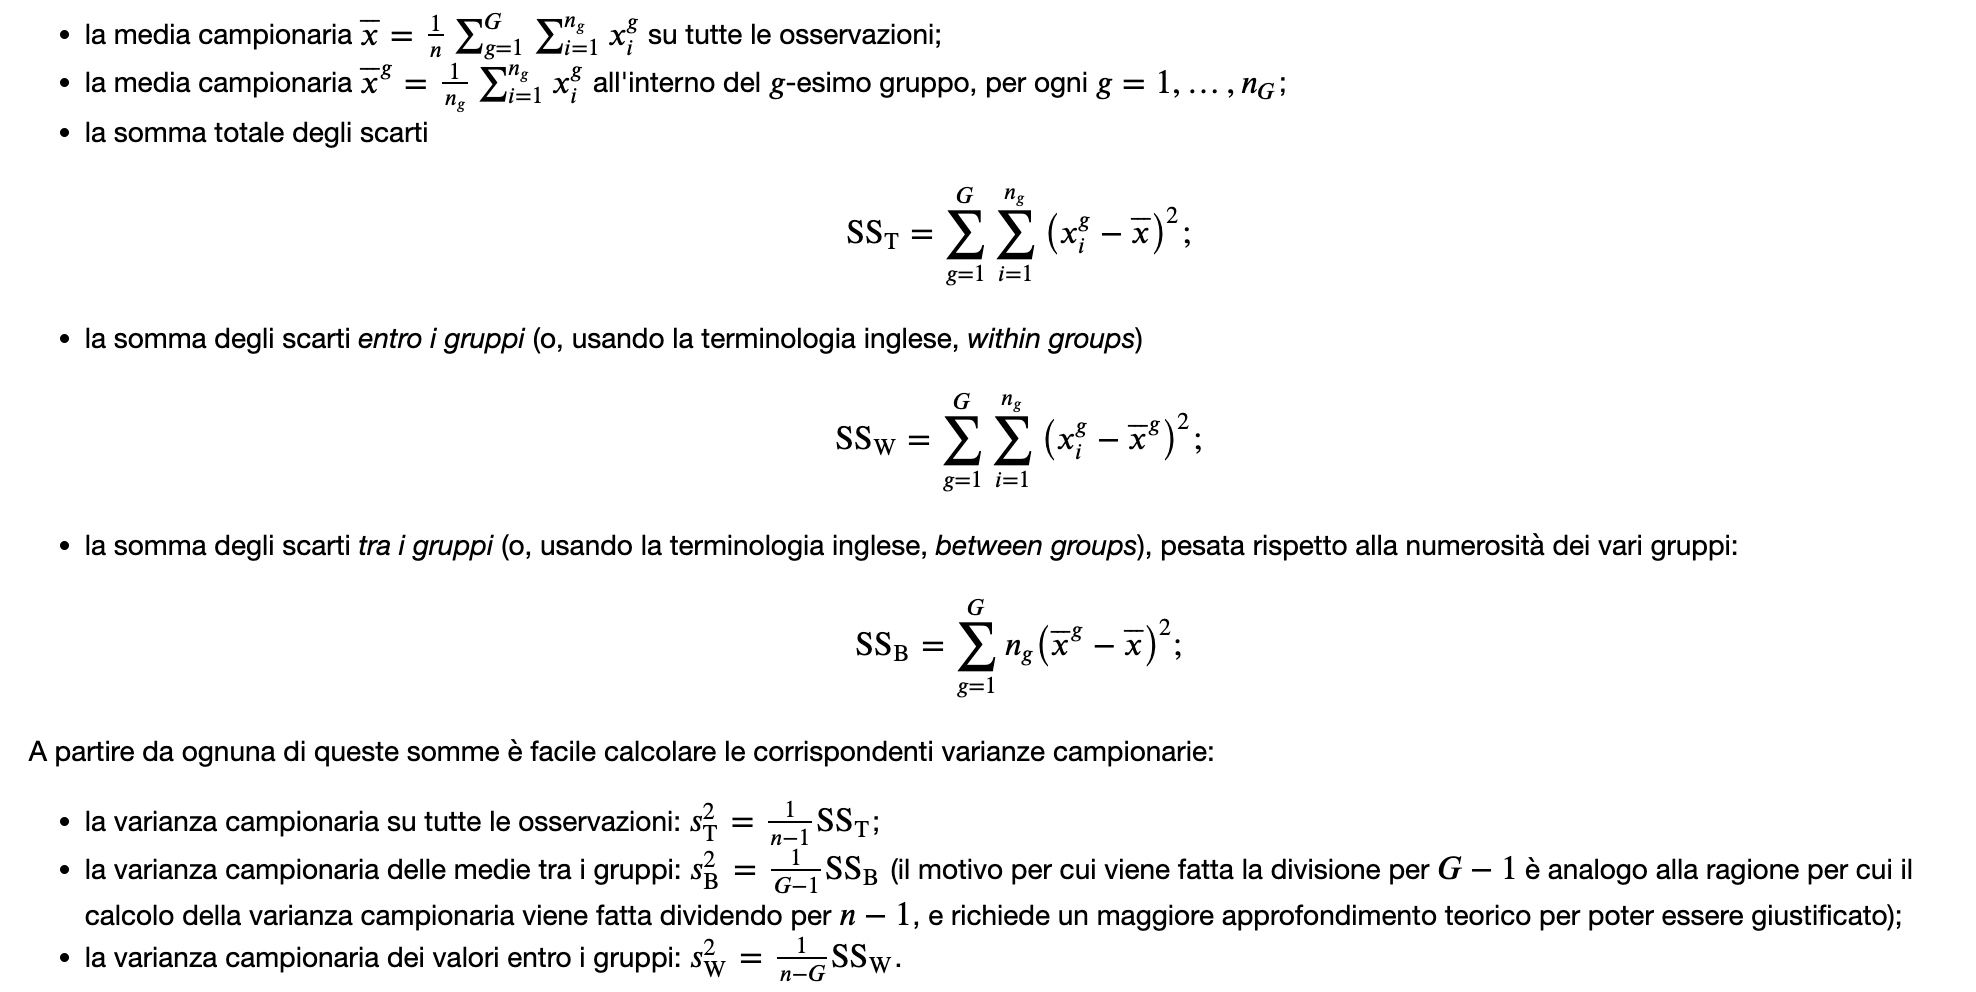
\includegraphics[scale=0.7]{anova}

E' possibile dimostrare che\begin{center}
$SS_T = SS_W + SS_B$
\end{center}





\section{Definizioni}
La definizione assiomatica della probabilità riassume in pochi punti quei concetti che si possono definire intuitivi nel calcolo delle probabilità.

\subsection{L'algebra degli eventi}
\begin{defin}
	Scelto un insieme $\Omega$ detto spazio campionario o degli eventi, si dice esito un elemento $\omega\in\Omega$ dell'insieme ed evento un suo sottoinsieme $E\subseteq\Omega$.

\end{defin}
\begin{defin}
	Sia $\A\in2^\Omega$ una collezione di sottoinsiemi di $\Omega$. Allora $\A$ è un'algebra se
	\begin{align*}
		 & \bullet ~ \Omega\in \A                                                                                            \\
		 & \bullet ~ \forall E\subseteq\Omega\qquad E\in\A\Rightarrow \bar E\in\A \qquad\text{con }\bar E:=\Omega\setminus E \\
		 & \bullet ~ \forall E_1,\dots E_n\in\Omega\qquad \forall i~E_i\in\A\Rightarrow \bigcup\limits_{i=1}^n E_i \in\A
	\end{align*}
	$\A$ è una $\sigma$-algebra su $\Omega$ se l'ultima condizione si può estendere a unioni numerabili qualsiasi.
\end{defin}




\subsection{Assiomi di Kolmogorov}
La probabilità viene definita come una funzione di un'algebra degli eventi $\A$ in $\R$:
\begin{equation*}
	P:\A\to\R
\end{equation*}

I seguenti assiomi, detti di Kolmogorov, decretano le proprietà che la probabilità rispetta:


\subsubsection{Primo assioma}
L'immagine di $P$ è l'insieme $[0,1]\in\R$. Equivalentemente, la probabilità di qualunque evento è compresa tra $0$ e $1$:
\begin{equation*}
	\forall E\in\A\qquad 0\leq P(E)\leq 1
\end{equation*}


\subsubsection{Secondo assioma}
La probabilità dello spazio campionario è $1$:
\begin{equation*}
	P(\Omega)=1
\end{equation*}


\subsubsection{Terzo assioma}
La probabilità dell'unione di eventi mutuamente esclusivi, cioè disgiunti (intuitivamente, il cui avvenire dell'uno esclude l'avvenire dell'altro), è uguale alla somma delle probabilità dei singoli:
\begin{equation*}
	\forall E_1,\dots,E_n\in\A\qquad \forall i,j~E_i\cap E_j = \emptyset \Rightarrow P\left( \bigcup_{i=1}^n E_i \right)=\sum_{i=1}^n P(E_i)
\end{equation*}



\subsection{Teoremi elementari}
Dagli assiomi di Kolmogorov derivano alcune proprietà elementari facilmente dimostrabili.


\subsubsection{Probabilità dell'evento complementare}
\begin{defin}
	Dato un evento $E\in\A$, l'evento complementare è l'evento $\bar E := \Omega\setminus E$.
\end{defin}
\begin{teor}[probabilità dell'evento complementare] \label{t:probcompl}
	Dato un evento $E$, se la probabilità di $E$ è $P(E)$, la probabilità dell'evento complementare di $E$ è $1-P(E)$:
	\begin{equation*}
		\forall E\in\A\qquad P(\bar E)=1-P(E)
	\end{equation*}
\end{teor}
\begin{proof}
	\begin{align*}
		  & \left.
		\begin{array}{cc}
			E\cap\bar E=\emptyset \\
			E\cup\bar E=\Omega
		\end{array} \right\}  \bc{definizione di evento complementare} \\
		1 & = P(\Omega)        \bc{secondo assioma}                                  \\
		  & = P(E\cup\bar E)                                                         \\
		  & = P(E)+P(\bar E)   \bc{terzo assioma}
	\end{align*}
	ergo:
	\begin{equation*}
		P(\bar E)=1-P(E) \qedhere
	\end{equation*}
\end{proof}

\subsubsection{Probabilità dell'unione}
\begin{teor} \label{t:probunion}
	Dati due eventi $E,F\in\A$, la probabilità della loro unione è uguale alla somma delle loro probabilità meno la probabilità dell'intersezione:
	\begin{equation*}
		\forall E,F \in\A\qquad P(E\cup F)=P(E)+P(F)-P(E\cap F)
	\end{equation*}
\end{teor}
\begin{proof}
	L'unione degli eventi è scrivibile come l'unione di due insiemi disgiunti:
	\begin{equation*}
		E\cup F=E \cup (\bar E\cap F) \\[1ex]
	\end{equation*}

	Passando alle probabilità:
	\begin{align*}
		P(E\cup F) & = P(E)+P(\bar E\cap F)                                               \\
		           & = P(E)+P(\bar E\cap F)+P(E\cap F)-P(E\cap F)                         \\
		           & = P(E)+P((\bar E\cap F)\cup (E\cap F))-P(E\cap F) \bc{terzo assioma} \\
		           & = P(E)+P(F)-P(E\cap F)                            \qedbc
	\end{align*}
\end{proof}

\subsubsection{Probabilità dell'evento vuoto}
La probabilità dell'evento vuoto ($\emptyset$) è $0$. Un evento con probabilità nulla viene detto evento impossibile.
\begin{equation*}
	P(\emptyset)=0
\end{equation*}

\begin{proof}
	\begin{align*}
		P(\Omega)    & = 1 \bc{secondo assioma}                       \\
		P(\emptyset) & = P(\bar\Omega)                                \\
		             & = 1 - P(\Omega) \bc{teorema \ref{t:probcompl}} \\
		             & = 1 - 1 = 0     \qedbc
	\end{align*}
\end{proof}



\subsection{Spazi di probabilità}
\begin{defin}
	Uno spazio di probabilità è una tripla $(\Omega,\A,P)$ composta da uno spazio campionario $\Omega$, un'algebra degli eventi $\A$ e una funzione di probabilità $P$.
\end{defin}


\subsubsection{Spazi equiprobabili}
\begin{defin}
	Uno spazio è equiprobabile se gli eventi elementari (cioè corrispondenti a singoletti) hanno probabilità costante $p$.
\end{defin}

Un evento elementare è composto da un singolo esito, cioè è un singoletto dell'insieme delle parti dello spazio campionario.
\begin{teor}
	In uno spazio equiprobabile, la probabilità di ogni evento elementare $e$ è uguale al reciproco del numero $n$ degli eventi elementari (che sono ovviamente a due a due disgiunti):
	\begin{equation}
		P(e)=\frac{1}{n}
	\end{equation}
\end{teor}
\begin{proof}
	\begin{align*}
		1=P(\Omega)=P\left( \bigcup_{i=1}^n e_i \right) \bc{secondo assioma} \\
		=\sum_{i=1}^n P(e_i) = np \bc{terzo assioma}                         \\
	\end{align*}
	Ergo:
	\begin{equation*}
		\forall e_i ~ P(e_i)=p=\frac{1}{n} \qedhere
	\end{equation*}
\end{proof}

Gli eventi non elementari possono essere espressi come unione di eventi elementari.
\begin{teor}
	In uno spazio equiprobabile, dato un evento $E=\{e_1,\dots,e_k\}$:
	\begin{equation}
		P(E)=\frac{|E|}{n}
	\end{equation}
\end{teor}
\begin{proof}
	\begin{equation*}
		P(E)= \sum_{i=1}^{|E|} P(e_i) = \frac{|E|}{n} \qedhere
	\end{equation*}
\end{proof}

%% Copyright (C) 2021 Alessandro Clerici Lorenzini
%
% This work may be distributed and/or modified under the
% conditions of the LaTeX Project Public License, either version 1.3
% of this license or (at your option) any later version.
% The latest version of this license is in
%   http://www.latex-project.org/lppl.txt
% and version 1.3 or later is part of all distributions of LaTeX
% version 2005/12/01 or later.
%
% This work has the LPPL maintenance status `maintained'.
%
% The Current Maintainer of this work is Alessandro Clerici Lorenzini
%
% This work consists of the files listed in work.txt


\section{Probabilità condizionata}
La probabilità condizionata vede protagonisti un evento condizionato e un evento condizionante e, concettualmente, restringe lo spazio campionario all'evento condizionante.

\begin{defin}
	La probabilità condizionata da un evento $F$ (evento condizionante) su un evento $E$ (evento condizionato) viene definita, quando $F$ non è impossibile (ossia per $P(F)\neq 0$), come segue:
	\begin{equation*}
		P(E\mid F)=\frac{P(E \cap F)}{P(F)}
	\end{equation*}
\end{defin}


Dalla definizione di probabilità condizionata deriva la seguente \textbf{regola di fattorizzazione}:
\begin{equation} \label{eq:regfatt}
	P(E \cap F)=P(E\mid F)\cdot P(F)
\end{equation}



\subsection{Teorema delle probabilità totali}

\subsubsection{Caso particolare}
Dati eventi $E, F\in \A$, l'evento $E$ può essere scritto come la parte di $E$ che non contiene elementi di $F$, ossia $E\cap \bar F$, unita disgiuntamente alla parte che ne contiene, ossia $E \cap F$:
\begin{align*}
	(E \cap \bar F) \cap (E \cap F) & = E \cap (F \cap \bar F)\bc{proprietà distributiva}  \\
	                                & = E \cap \emptyset = \emptyset                       \\[2ex]
	(E \cap \bar F) \cup (E \cap F) & = E \cap (F \cup \bar F) \bc{proprietà distributiva} \\
	                                & = E \cap \Omega = E
\end{align*}

Avendo espresso $E$ come unione di eventi disgiunti, si può applicare il terzo assioma:
\begin{equation*}
	P(E) = P((E \cap \bar F)\cup(E \cap F)) = P(E \cap \bar F)+P(E \cap F)
\end{equation*}
e, per la regola \eqref{eq:regfatt} di fattorizzazione, assunto $P(F)\neq 0 \land P(\bar F)\neq 0$:
\begin{equation*}
	=P(E\mid \bar F)\cdot P(\bar F) + P(E \mid F)\cdot P(F)
\end{equation*}

\subsubsection{Forma generale}
\begin{teor}[delle probabilità totali]
	Data una partizione di $\Omega$ composta da eventi non impossibili $F_1,\dots, F_n$ e un evento $E$:
	\begin{equation*}
		P(E)= \sum_{i=1}^n P(E \mid F_i)\cdot P(F_i)
	\end{equation*}
\end{teor}
\begin{proof}
	La dimostrazione avviene in analogia con il caso particolare. Questa volta, tuttavia, gli eventi della partizione sono disgiunti per ipotesi e non in quanto complementari:
	\begin{equation*}
		P(E)=P \left(\bigcup_{i=1}^n (E\cap F_i) \right) = \sum_{i=1}^n P(E\cap F_i) = \sum_{i=1}^n P(E \mid F_i)\cdot P(F_i) \qedhere
	\end{equation*}
\end{proof}


%1:13:15

\subsection{Teorema di Bayes}
Nelle stesse ipotesi del teorema delle probabilità totali si dimostra un altro teorema, detto di Bayes:
\begin{teor}[di Bayes]
	Data una partizione di $\Omega$ composta da eventi non impossibili $F_1,\dots, F_n$ e un evento $E$:
	\begin{equation*}
		P(F_j\mid E)=\frac{P(E\mid F_j)\cdot P(F_j)}{\sum\limits_{i=1}^n P(E \mid F_i)\cdot P(F_i)}
	\end{equation*}
\end{teor}

\begin{proof}
	\begin{equation*}
		P(F_j\mid E)=\frac{P(F_j \cap E)}{P(E)}=\frac{P(E\mid F_j)\cdot P(F_j)}{\sum\limits_{i=1}^n P(E \mid F_i)\cdot P(F_i)} \qedhere
	\end{equation*}
\end{proof}



\subsection{Eventi indipendenti}
\begin{defin}
	Eventi $E$ e $F$, con $P(F)>0$, si dicono indipendenti se $P(E \mid F)=P(E)$
\end{defin}

Equivalentemente, per definizione di probabilità condizionata
\begin{gather*}
	\frac{P(E \cap F)}{P(F)}=P(E) \\[1ex]
	P(E \cap F)=P(E)\cdot P(F)
\end{gather*}
e ovviamente, se $P(E)>0$:
\begin{equation*}
	P(F \mid E)=P(F)
\end{equation*}

\subsubsection{Proprietà}
\begin{teor}
	Se $E$ e $F$ sono indipendenti, allora $E$ e $\bar F$ sono indipendenti.
\end{teor}
\begin{proof}
	\begin{equation*}
		E = (E\cap F) \cup (E \cap \bar F)
	\end{equation*}
	\begin{align*}
		P(E \cap \bar F) & = P(E) - P(E \cap F)    \bc{terzo assioma}                          \\
		                 & = P(E) - P(E)\cdot P(F) \bc{in quanto $E$ ed $F$ sono indipendenti} \\
		                 & = P(E)(1-P(F))                                                      \\
		                 & = P(E)\cdot P(\bar F)   \bc{teorema \ref{t:probcompl}} \qedhere
	\end{align*}
\end{proof}

\subsubsection{Tripla di eventi indipendenti}
\begin{defin}
	Tre eventi $E$, $F$, $G$ sono indipendenti se
	\begin{itemize}
		\item $P(E \cap F)=P(E)\cdot P(F)$
		\item $P(E \cap G)=P(E)\cdot P(G)$
		\item $P(F \cap G)=P(F)\cdot P(G)$
		\item $P(E \cap F \cap G)=P(E)\cdot P(F)\cdot P(G)$
	\end{itemize}
\end{defin}

\noindent
Per quanto riguarda $E$, $F\cup G$:
\begin{align*}
	P(E \cap & (F\cup G))  = P((E\cap F)\cup (E\cap G))                \bc{distributiva}              \\
	         & = P(E \cap F) + P(E\cap G) - P((E\cap F)\cap (E\cap G)) \bc{teorema \ref{t:probunion}} \\
	         & = P(E)P(F) + P(E)P(G) - P(E)P(F)P(G)                    \bc{indipendenza}              \\
	         & = P(E)(P(F) + P(G)-P(F)P(G))
\end{align*}

\subsubsection{\texorpdfstring{$n$}{n}-upla di eventi indipendenti}
\begin{defin}[$n$-upla di eventi indipendenti]
	Eventi $E_1,\dots,E_n$ si dicono indipendenti se e solo se comunque apportata su di essi una selezione di $r$ eventi la probabilità dell'intersezione degli eventi selezionati è uguale al prodotto della probabilità dei singoli.
	\begin{equation*}
		\forall r<n\in\mathbb{N}~\forall~1\leq \alpha_1 \leq\dots\leq\alpha_r\leq n \qquad P \left(\bigcap_{i=1}^r E_{\alpha_i} \right)=\prod_{i=1}^r P(E_{\alpha_i})
	\end{equation*}
\end{defin}

\begin{examp}
	Dato un sistema in serie di dimensione $n$:
	\begin{gather*}
		\forall i=1,\dots,n \qquad p_i=P(\text{l'}i\text{-esimo componente funziona}) \\[1ex]
		P(\text{il sistema funziona}) = P(\text{tutti i componenti funzionanno}) = \\
		P\left(\bigcap_{i=1}^n \text{l'}i\text{-esimo componente funziona}\right)
	\end{gather*}

	In un sistema in parallelo:
	\begin{gather*}
		P(\text{il sistema funziona}) = 1-P(\text{il sistema non funziona}) = \\[1ex]
		1-P(\text{tutti i componenti non funzionano}) = \\[1ex]
		1- P\left(\bigcap_{i=1}^n \text{l'}i\text{-esimo componente non funziona}\right) = \\[1ex]
		1-\prod_{i=1}^n P(\text{l'}i\text{-esimo componente non funziona}) =
		1-\prod_{i=1}^n 1-p_i =
	\end{gather*}
\end{examp}

%todo: BEYES fino a variabili aleatorie discrete
%% Copyright (C) 2021 Alessandro Clerici Lorenzini
%
% This work may be distributed and/or modified under the
% conditions of the LaTeX Project Public License, either version 1.3
% of this license or (at your option) any later version.
% The latest version of this license is in
%   http://www.latex-project.org/lppl.txt
% and version 1.3 or later is part of all distributions of LaTeX
% version 2005/12/01 or later.
%
% This work has the LPPL maintenance status `maintained'.
%
% The Current Maintainer of this work is Alessandro Clerici Lorenzini
%
% This work consists of the files listed in work.txt


\section{Variabili aleatorie discrete}
\begin{defin}
	In uno spazio di probabilità $(\Omega, \A, p)$, una variabile aleatoria (o casuale) è una funzione\footnote{in verità, la funzione deve soddisfare il criterio: $\{\omega \mid X(\omega)\leq r\}\in\A\quad\forall r\in\R$} $X:\Omega\to \R$.
	L'immagine di una variabile aleatoria $(x_1, ... x_n)$ si dice supporto e si indica con $D_X$ (dominio). Ogni elemento del supporto, cioè l'immagine per $X$ di un elemento di $\Omega$, si dice specificazione. Una specificazione generica di $X$ si indica tipicamente con $x$.
\end{defin}


\subsection{Definizioni}
\begin{defin}
	Una variabile aleatoria è discreta se e solo se il suo supporto è numerabile.
\end{defin}

\begin{examp}
	Se $\Omega$ è l'insieme di esiti del lancio di due dadi, una possibile variabile aleatoria $X$ è la somma degli esiti dei due dadi. In questo caso immagini di $X$ non sono equiprobabili. Se invece per $X$ si sceglie il valore del primo dado, le immagini sono equiprobabili.
\end{examp}

\begin{defin}[funzione indicatrice]
	Siano $A$ e $D$ insiemi tali che $A\subseteq D$. La funzione indicatrice (o caratteristica) di $A$ rispetto a $D$ è la funzione $I:D\to \{0,1\}$ che associa a un elemento di $D$ il numero $1$ se l'elemento appartiene ad $A$, o $0$ altrimenti:
	\begin{equation*}
		I_A(x) := \begin{cases}
			1 \qquad x\in A \\
			0 \qquad x\notin A
		\end{cases}
	\end{equation*}
\end{defin}

\begin{defin}[funzione indicatrice di un evento] \label{def:findiceven}
	La funzione indicatrice di un evento $A$ è la variabile aleatoria che ha specificazione $1$ se l'evento $A$ si verifica e $0$ se l'evento non si verifica.
\end{defin}



\subsection{Funzione di ripartizione}
\begin{defin}[funzione di ripartizione] \label{def:fripar}
	Data una variabile aleatoria $X$, la funzione di ripartizione (o di distribuzione cumulativa) $F_X:\R\to[0,1]$ è la funzione che associa a un valore $x\in\R$ la probabilità che l'esito di $X$ ne sia minore o uguale:
	\begin{equation*}
		\forall x\in\R\quad F_X(x):=P(X\leq x)
	\end{equation*}
\end{defin}

La funzione di ripartizione si annulla quandunque l'input è minore della minima specificazione.




\subsection{Funzione di massa di probabilità}
\begin{defin}[funzione di massa di probabilità] \label{def:fmassaprob}
	Data una variabile aleatoria discreta $X$, la funzione di massa di probabilità $p_X:\R\to[0,1]$ è la funzione che associa a un valore $x\in\R$ la probabilità che l'esito di $X$ sia uguale a $x$:
	\begin{equation*}
		\forall x \in\R\quad p_X(x)= P(x=X)
	\end{equation*}
\end{defin}

La somma delle immagini della funzione di massa di probabilità per tutte le specificazioni di $X$ è ovviamente uguale a $1$:
\begin{equation} \label{eq:sommamassa}
	\sum_i p_X (x_i) = 1
\end{equation}

La funzione di massa di probabilità di $X$ si annulla nei punti di $\R$ non appartenenti al supporto di $X$, in particolare essendo la funzione di massa di probabilità fissata sul $\R$ e non su $D$, possiamo dire che se un evento non appartiene a $D$, il suo valore sarà sicuramente uguale a 0.

\begin{prop}
	Per le variabili aleatorie discrete vale la seguente relazione tra la funzione di ripartizione e la funzione di massa di probabilità:
	\begin{equation*}
		F_X(x)=\sum_{a\leq x} p_X(a)
	\end{equation*}
	con $a\in D_X$.
\end{prop}
\begin{proof}
	\begin{align*}
		F_X(x) & = P(X\leq x)                             \bc{definizione \ref{def:fripar}}     \\
		       & = P\left(\bigcup_{a\leq x}\{X=a\}\right)                                       \\
		       & = \sum_{a\leq x} P(X=a)                  \bc{unione di eventi disgiunti}       \\
		       & = \sum_{a\leq x} p_X(a)                  \bc{definizione \ref{def:fmassaprob}}
	\end{align*}
\end{proof}
Se conosco la funzione di massa di probabilità sono in grado di calcolare della funzione di ripartizione. Andiamo a vedere tuttavia il contrario:
A partire dalla funzione di partizione riusciamo a dire qualcosa sulla funzione di massa di probabilitòà?
\begin{equation*}
	F_x \rightarrow P_x
	\end{equation*}
$P_x(x) = P(X = x) = P(x' < x \leq x)= f_x( $ TODO
Si, il contenuto informativo della funzione di massa di probabilità e della funzione di ripartizione è la medesima; conoscendo una possiamo calcolare l'altra.




\subsection{Valore atteso}
Il valore atteso di una variabile aleatoria $X$ è un indice di centralità delle specificazioni della variabile aleatoria.
\begin{defin}[valore atteso] \label{def:valatt}
	Data una variabile aleatoria discreta $X$, il valore atteso di $X$ è la media delle specificazioni di $X$ pesata con le rispettive probabilità:
	\begin{equation*}
		\ev{X}=\sum_i x_i P(X=x_i)
	\end{equation*}
	Talvolta si usa anche la notazione $\mu=\mu_X=\ev{X}$.
\end{defin}
\noindent
In generale, non è detto che la sommatoria che definisce il valore atteso converga.

\begin{prop} \label{prop:indvalatt}
	Il valore atteso della funzione indicatrice di un evento è uguale alla probabilità dell'evento:
	\begin{equation*}
		\ev{I_A}=P(A)
	\end{equation*}
\end{prop}
\begin{proof}
	Applicando la definizione \ref{def:valatt} di valore atteso e la \ref{def:findiceven} di funzione indicatrice di un evento:
	\begin{equation*}
		\ev{I_A}=1*P(A)+0*(1-P(A))=P(A)
	\end{equation*}
\end{proof}

\subsubsection{Linearità del valore atteso}
\begin{prop}
	Il valore atteso di una variabile aleatoria discreta $X$ è lineare rispetto a una trasformazione lineare $ax+b$ applicata alle specificazioni $x_i$ di $X$:
	\begin{equation*}
		D_Y = \{ax_i+b \mid x_i\in D_X\} \qquad\Rightarrow\qquad \ev{Y}=a\ev{X}+b
	\end{equation*}
	Si scrive anche $Y=aX+b$.
\end{prop}
\begin{proof}
	Poiché le probabilità per le rispettive specificazioni rimangono invariate:
	\begin{align*}
		\ev{Y} & = \sum_i (a x_i + b) P(X=x_i)                                                    \\
		       & = a\sum_i x_i P(X=x_i) + b\sum_i P(X=x_i)                                        \\
		       & = a\underbrace{\sum_i x_i p_X(x_i)}_{\ev{x}} + b\underbrace{\sum_i p_X(x_i)}_{1} \\
		       & = a \ev{x} + b \bc{\eqref{eq:sommamassa} e definizione \ref{def:valatt}}
	\end{align*}
\end{proof}



\subsection{Varianza di una variabile aleatoria}
\begin{defin}[varianza di una variabile aleatoria] \label{def:var}
	La varianza di una variabile aleatoria $X$ è definita come segue:
	\begin{equation*}
		\var(X) = \sigma^2_X := \ev{(X-\ev{X})^2}
	\end{equation*}
\end{defin}
Ed è rappresentata dal quadrato della differenza degli scarti. Sarà talvolta tuttavia più comodo utilizzare la formula in $(5)$.



\begin{defin}[deviazione standard di una variabile aleatoria]
	La deviazione standard di una variabile aleatoria $X$ è così definita:
	\begin{equation*}
		\sigma(X) = \sigma_X :=\sqrt{\var(X)}
	\end{equation*}
\end{defin}


\subsubsection{Proprietà della varianza}
\begin{prop} \label{prop:varalt}
	La varianza di $X$ può essere espressa equivalentemente come la differenza tra il valore atteso del quadrato di $X$ e il valore atteso al quadrato di $X$:
	\begin{equation} \label{eq:varalt}
		\var(X) = \ev{X^2}- \ev{X}^2
	\end{equation}
\end{prop}
\begin{proof}
	\begin{align*}
		\var(X) & = \ev{(X-\ev{X})^2}          \bc{definizione \ref{def:var}}   \\
		        & = \ev{X^2-2\mu X+\mu^2}      \bc{sviluppando il quadrato}     \\
		        & = \ev{X^2}-2\mu \ev{X}+\mu^2 \bc{linearità del valore atteso} \\
		        & = \ev{X^2}-2\mu^2+\mu^2      \bc{definizione di $\mu$}        \\
		        & = \ev{x^2}- \ev{x}^2
	\end{align*}
\end{proof}

\begin{prop} \label{prop:indvar}
	La varianza della funzione indicatrice di un evento $A$ è uguale al prodotto delle probabilità di $A$ e del suo complementare:
	\begin{equation*}
		\var(I_A) = P(A)P(\bar A)
	\end{equation*}
\end{prop}
\begin{proof}
	\begin{align*}
		\var(I_A) & = \ev{I_A^2}- \ev{I_A}^2                             \\
		          & = \ev{I_A}- \ev{I_A}^2   \bc{idempotenza di $I_A$}   \\
		          & = \ev{I_A}(1- \ev{I_A})  \bc{proprietà distributiva} \\
		          & = P(A)P(\bar A)
	\end{align*}
\end{proof}

\begin{prop}
	In una trasformazione lineare su una variabile aleatoria $X$, una traslazione non influisce sulla varianza; al contrario, una dilatazione si traduce in una dilatazione quadratica.
	\begin{equation*}
		\var(aX+b)=a^2\var(X)
	\end{equation*}
\end{prop}
\begin{proof}
	\begin{align*}
		\var(aX+b) & = \ev{(aX+b-\ev{aX+b})^2} \\
		           & = \ev{(aX+b-a\ev{X}-b)^2} \\
		           & = \ev{(a(X-\ev{X}))^2}    \\
		           & = a^2~\ev{(X-\ev{X})^2}   \\
		           & = a^2 \var(X)             \\
	\end{align*}
\end{proof}
Bisogna notare che, come nella varianza campionaria, il valore $b$ è ininfluente.\\
Jump to \ref{Multivariati}


\subsection{Funzione di ripartizione congiunta}
\begin{defin}
	Data una coppia di variabili aleatorie $X, Y$, la funzione di ripartizione congiunta $F_X:\R\times\R\to[0,1]$ (o di distribuzione cumulativa congiunta) è la funzione che associa a una coppia di valori reali per $x$ e $y$ la probabilità che l'esito di $X$ sia minore o uguale a $x$ e l'esito di $Y$ sia minore o uguale a $y$:
	\begin{equation*}
		\forall x,y\in\R\qquad F_{X,Y}(x,y):=P(X\leq x, Y\leq y) \\
	\end{equation*}
\end{defin}

Il limite per $y$ che tende a $+\infty$ della funzione di ripartizione congiunta di $X$ e $Y$ è uguale alla funzione di ripartizione di $X$. In questo caso si dice che $F_X(x)$ è la distribuzione marginale rispetto a $X$:
\begin{equation} \label{eq:distrmargin}
	\lim_{y\to+\infty}F_{X,Y}(x, y) = \lim_{y\to+\infty}P(X\leq x,Y\leq y) = P(X\leq x) = F_X(x)
\end{equation}
Analogo vale, ovviamente, per $x\to+\infty$.



\subsection{Funzione di massa di probabilità congiunta}
\begin{defin}
	Data una coppia di variabili aleatorie $X, Y$, la funzione di massa di probabilità congiunta $p_{X,Y}:\R\times\R\to[0,1]$ è la funzione che associa a una coppia di valori reali per $x$ e $y$ la probabilità che l'esito di $X$ sia uguale a $x$ e quello di $Y$ sia uguale a $y$:
	\begin{equation*}
		p_{X,Y}(x,y)=P(X=x,Y=y)
	\end{equation*}
\end{defin}

Analogamente a quanto visto nella \eqref{eq:distrmargin} con il limite, la somma per tutte le specificazioni $y_j$ di $Y$ di $p_{X,Y}(x,y_j)$ è uguale alla massa di probabilità marginale rispetto a $X$:
\begin{equation} \label{eq:massamargin}
	\sum_j p_{X,Y}(x,y_j) = p_X(x)
\end{equation}




\subsection{Indipendenza}
\begin{defin}
	Variabili aleatorie $X$ e $Y$ sono indipendenti se e solo se
	\begin{equation*}
		\forall A,B\subseteq\R\qquad P(X\in A, Y\in B)=P(X\in A)P(Y\in B)
	\end{equation*}
\end{defin}

La definizione è equivalente alla seguente proprietà della funzione di massa di probabilità congiunta:
\begin{prop}
	Variabili aleatorie $X$ e $Y$ sono indipendenti se e solo se
	\begin{equation*}
		a,b\in\R\qquad p_{X,Y}(a,b)=p_X(a)p_Y(b)
	\end{equation*}
\end{prop}
\begin{proof}
	L'implicazione verso destra:
	\begin{gather*}
		\forall A,B\subseteq\R\qquad P(X\in A, Y\in B)=P(X\in A)P(Y\in B) \\
		\Rightarrow \\
		a,b\in\R\qquad p_{X,Y}(a,b)=p_X(a)p_Y(b)
	\end{gather*}
	è immediata dal momento che si possono scegliere sottoinsiemi di $\R$ corrispondenti a singoletti contenenti $a$ e $b$ ($A=\{a\}$ e $B=\{b\}$).

	L'implicazione inversa parte dalla ricostruzione di $A$ e $B$ come unioni di singoletti:
	\begin{align*}
		P(X\in A, Y\in B) & = \sum_{a\in A}\sum_{b\in B} p_{X,Y}(a,b)                           \\
		                  & = \sum_{a\in A}\sum_{b\in B} p_X(a)p_Y(b) \bc{ipotesi}              \\
		                  & = \left(\sum_{a\in A}p_X(a)\right)\left(\sum_{b\in B} p_Y(b)\right) \\
		                  & = P(X\in A)P(Y\in B)
	\end{align*}
\end{proof}

Si dimostra anche la seguente equivalenza:
\begin{prop}
	Variabili aleatorie $X$ e $Y$ sono indipendenti se e solo se
	\begin{equation*}
		a,b\in\R\qquad F_{X,Y}(a,b)=F_X(a)F_Y(b)
	\end{equation*}
\end{prop}



\subsection{Multivariati}\label{Multivariati}
I concetti visti per coppie di variabili aleatorie si estendono a vettori aleatori (più comunemente detti variabili aleatorie multivariate, o multivariati) di dimensione arbitraria:


\subsubsection{Funzione di ripartizione}
\begin{defin}
	Date $n$ variabili aleatorie $X_1, \dots, X_n$, la funzione di ripartizione $F_{X_1,\dots,X_n}:\R^n\to[0,1]$ è la funzione che associa a una $n$-upla di valori reali $x_1,\dots,x_n$ la probabilità che l'esito di $X_i$ sia minore o uguale a $x_i$ per ogni $i$ da $1$ a $n$:
	\begin{equation*}
		F_{X_1,\dots,X_n}(x_1,\dots,x_n) = P(X_1\leq x_1,\dots,X_n\leq x_n)
	\end{equation*}
\end{defin}

\subsubsection{Funzione di ripartizione congiunta}
Date $m, n$ variabili aleatorie, la funzione di ripartizione congiunta è rappresentata da:
\begin{center}
$F_{(x,y)} (x,y) := P(X \leq x_i, Y \leq y)$
\end{center}
Il limite della funzione di ripartizione congiunta è invece rappresentata da:
\begin{center}
$\lim_{y\to\infty} F_{(x,y)} (x,y) =$ \\
$\lim_{y\to\infty} P(X \leq x, Y \leq y) = $\\
$P(X \leq x) = F_x(x)$
\end{center}
Ovvero la funzione di ripartizione marginale di $x$.

\subsubsection{Funzione di massa di probabilità congiunta}
\begin{defin}
	Date $n$ variabili aleatorie $X_1, \dots, X_n$, la funzione di massa di probabilità $p_{X_1,\dots,X_n}:\R^n\to[0,1]$ è la funzione che associa a una $n$-upla di valori reali $x_1,\dots,x_n$ la probabilità che l'esito di $X_i$ sia uguale a $x_i$ per ogni $i$ da $1$ a $n$:
	\begin{equation*}
		p_{X_1,\dots,X_n}(x_1,\dots,x_n) = P(X_1=x_1,\dots,X_n=x_n)
	\end{equation*}
\end{defin}
%TODO: RECHECK FROM HERE

Considerando la funzione di ripartizione congiunta:
\begin{center}
$P_{x,y} (x,y) = P(X = x, Y = y)$
\end{center}
Funzione di massa di probabilità marginale rappresentata da:
\begin{center}
$\sum_{x} P_{x,y} (x,y) = P_x(y)$
\end{center}

\subsubsection{Indipendenza}
Finora il concetto d'indipendenza l'abbiamo considerata solo per l'indipendenza tra eventi, vediamo ora se è possibile rappresentare questo concetto nelle variabili aleatore. L'indipendenza è imporatnte perché se verifica, ci permette di effettuare numerose fattorizzazioni significative.
\begin{defin}
	Variabili aleatorie $X_1,\dots,X_n$ sono indipendenti se e solo se
	\begin{equation*}
		\forall A_1,\dots,A_n\subseteq\R \qquad P\left(\bigland_{i=1}^n X_i\in A_i\right) = \prod_{i=1}^n P(X_i\in A_i)
	\end{equation*}
\end{defin}



\subsubsection{Valore atteso}
Il valore atteso per una funzione applicata a una coppia di variabili aleatorie discrete coinvolge tutte le combinazioni\footnote{la sommatoria con doppio indice può essere scomposta in due sommatorie, una per ogni indice} di specificazioni delle due variabili:
\begin{equation*}
	\ev{f(x,y)}=\sum_{i,j}f(x_i,y_j)P(X=x_i,Y=y_i)
\end{equation*}

\begin{prop}
	Il valore atteso della somma di due variabili aleatorie discrete è uguale alla somma dei valori attesi delle stesse.
	\begin{equation*}
		\ev{X+Y}=\ev{X}+\ev{Y}
	\end{equation*}
\end{prop}
\begin{proof}
	\begin{align*}
		\ev{X+Y} & = \sum_i\sum_j (x_i+y_j) P(X=x_i,Y=y_j)                               \\
		         & = \sum_i\sum_j x_i P(X=x_i,Y=y_j) + \sum_i\sum_j y_j P(X=x_i,Y=y_j)   \\
		         & = \sum_i x_i \sum_j P(X=x_i,Y=y_j) + \sum_j y_j \sum_i P(X=x_i,Y=y_j)
	\end{align*}
	Le due sommatorie interne sono probabilità marginali:
	\begin{align*}
		 & = \sum_i x_i P(X=x_i) + \sum_j y_i P(Y=y_i) \\
		 & = \ev{X} + \ev{Y}
	\end{align*}
\end{proof}

Generalizzando:
\begin{prop}
	Il valore atteso della somma di variabili aleatorie discrete è uguale alla somma dei valori attesi delle stesse.
	\begin{equation*}
		\ev{\sum_i X_i}=\sum_i \ev{X_i}
	\end{equation*}
\end{prop}

Di conseguenza, se si può esprimere una variabile $X$ come la somma di variabili $X_1,\dots,X_n$, è sufficiente calcolare il valore atteso di ciascuna componente per calcolare quello della variabile iniziale.


\subsubsection{Altre proprietà}
Il seguente risultato è una generalizzazione della varianza, utile a valutare quanto un'approssimazione $c$ di $X$ è buona. La migliore approssimazione è $c=\ev{X}$, in coerenza con l'interpretazione semantica di $\ev{X}$.
\begin{prop}
	\begin{equation*}
		\ev{(X-c)^2}=\var(X)+(\mu-c)^2\geq\var(X)
	\end{equation*}
\end{prop}
\begin{proof}
	Se $\mu=\ev{X}$
	\begin{align*}
		\ev{(X-c)^2} & = \ev{(X-\mu+\mu-c)^2}                                                     \\
		             & = \ev{(X-\mu)^2-2(X-\mu)(\mu-c)+(\mu-c)^2}                                 \\
		             & = \ev{(X-\mu)^2}-\ev{2(X-\mu)(\mu-c)}+(\mu-c)^2                            \\
		             & = \ev{(X-\mu)^2}-2(\mu-c)\underbrace{\ev{X-\mu}}_{=\ev{X}-\mu=0}+(\mu-c)^2 \\
		             & = \ev{(X-\mu)^2}+(\mu-c)^2
	\end{align*}
\end{proof}



\subsection{Covarianza}

\begin{defin}
	Date due variabili aleatorie $X$ e $Y$, la covarianza tra $X$ e $Y$ è così definita:
	\begin{equation} \label{eq:covar}
		\cov(X,Y)=\ev{(X-\mu_X)(Y-\mu_Y)}
	\end{equation}
\end{defin}
\noindent
Ovviamente la covarianza è simmetrica, ossia $\cov(X,Y)=\cov(Y,X)$.


\subsubsection{Proprietà}
La seguente è una definizione equivalente per la covarianza tra due variabili aleatorie:
\begin{prop} \label{prop:covalt}
	Date due variabili aleatorie $X$ e $Y$, la covarianza tra $X$ e $Y$ è uguale al valore atteso del prodotto delle due meno il prodotto dei rispettivi valori attesi:
	\begin{equation*}
		\cov(X,Y)=\ev{XY}-\ev{X}\ev{Y}
	\end{equation*}
\end{prop}
\begin{proof}
	Sviluppando la \eqref{eq:covar}:
	\begin{align*}
		\cov(X,Y) & = \ev{XY-\mu_X Y-\mu_Y x + \mu_X\mu_Y}                                                            \\
		          & = \ev{X,Y}-\underbrace{\mu_X\ev{Y}}_{\mu_X\mu_Y}-\underbrace{\mu_Y\ev{X}}_{\mu_X\mu_Y}+\mu_X\mu_Y \\
		          & =\ev{XY}-\ev{X}\ev{Y}
	\end{align*}
\end{proof}

\begin{prop}
	La covarianza è lineare rispetto alla dilatazione di una variabile per una costante:
	\begin{equation*}
		\cov(aX,Y)=a\cov(X,Y)
	\end{equation*}
\end{prop}
\begin{proof}
	Applicando la proprietà \ref{prop:covalt}:
	\begin{align*}
		\cov(aX,Y) & = \ev{aXY}-\ev{aX}\ev{Y}  \\
		           & = a(\ev{XY}-\ev{X}\ev{Y}) \\
		           & = a\cov(X,Y)
	\end{align*}
\end{proof}

\begin{prop} \label{prop:covsum0}
	\begin{equation*}
		\cov(X+Y,Z)=\cov(X,Z)+\cov(Y,Z)
	\end{equation*}
\end{prop}
\begin{proof}
	\begin{align*}
		\cov(X+Y,Z) & = \ev{(X+Y)Z} - \ev{X+Y}\ev{Z}                    \\
		            & = \ev{XZ+YZ} - (\ev{X} + \ev{Y}) \ev{Z}           \\
		            & = \ev{XZ} + \ev{YZ} - \ev{X}\ev{Z} - \ev{Y}\ev{Z} \\
		            & = \cov(X,Z) + \cov(Y,Z)
	\end{align*}
\end{proof}

Generalizzando:
\begin{prop} \label{prop:covsum}
	\begin{equation*}
		\cov\left(\sum_i X_i,\sum_j Y_j\right)=\sum_i\sum_j\cov(X_i,Y_j)
	\end{equation*}
\end{prop}
\begin{proof}
	\begin{align*}
		\cov\left(\sum_i X_i,\sum_j Y_j\right) & = \sum_i\cov\left(X_i,\sum_j Y_j\right) \bc{proprietà \ref{prop:covsum0}} \\
		                                       & = \sum_i\sum_j \cov(X_i,Y_j) \bc{proprietà \ref{prop:covsum0}}            \\
	\end{align*}
\end{proof}

\begin{prop}
	La covarianza tra una variabile aleatoria $X$ e se stessa è uguale alla varianza di $X$:
	\begin{equation*}
		\cov(X,X)=\var(X)
	\end{equation*}
\end{prop}
\begin{proof}
	\begin{align*}
		\cov(X,X) & = \ev{(X-\mu)(X-\mu)} \\
		          & = \ev{(X-\mu)^2}      \\
		          & = \var(X)
	\end{align*}
\end{proof}

\begin{prop} \label{prop:varsum}
	La varianza della somma di due variabili aleatorie $X$ e $Y$ è uguale alla somma delle rispettive varianze più il doppio della loro covarianza:
	\begin{equation*}
		\var(X+Y) = \var(X)+\var(Y)+2\cov(X,Y)
	\end{equation*}
\end{prop}
\begin{proof}
	Usando la definizione alternativa (proprietà \ref{prop:varalt}):
	\begin{align*}
		\var(X+Y) & = \ev{(X+Y)^2} - \ev{X+Y}^2                                            \\
		          & = \ev{X^2+2XY+Y^2}-(\ev{X}+\ev{Y})^2                                   \\
		          & = \ev{X^2} + 2\ev{XY} + \ev{Y^2} - \ev{X}^2 - 2\ev{X}\ev{Y} - \ev{Y}^2 \\
		          & = \ev{X^2} - \ev{X}^2 + \ev{Y^2} - \ev{Y}^2 + 2(\ev{XY}-\ev{X}\ev{Y})  \\
		          & = \var(X) + \var(Y) + 2\cov(X,Y)
	\end{align*}
\end{proof}

Generalizzando:
\begin{prop} \label{prop:varsumcov}
	\begin{equation*}
		\var\left(\sum_{i=1}^n X_i\right) = \sum_{i=1}^n \var(X_i) + \sum_{i\neq j}\cov(X_i,Y_j)
	\end{equation*}
\end{prop}
\noindent

\begin{teor}
	Il valore atteso del prodotto di variabili aleatorie discrete indipendenti è uguale al prodotto dei rispettivi valori attesi:
	\begin{equation*}
		\ev{XY} = \ev{X}\ev{Y}
	\end{equation*}
\end{teor}
\begin{proof}
	\begin{align*}
		\ev{XY} & = \sum_i\sum_j x_i y_j P(X=x_i,Y=y_i)                              \\
		        & = \sum_i\sum_j x_i y_j P(X=x_i)P(Y=y_j)                            \\
		        & = \left(\sum_i x_i P(X=x_i)\right)\left(\sum_j y_j P(Y=y_j)\right) \\
		        & = \ev{X}\ev{Y}
	\end{align*}
\end{proof}

\begin{corol}
	La covarianza di due variabili aleatorie discrete indipendenti $X$ e $Y$ è nulla:
	\begin{equation*}
		\cov(X,Y) = 0
	\end{equation*}
\end{corol}
\begin{proof}
	\begin{align*}
		\cov(X,Y) & = \ev{XY}-\ev{X}\ev{Y}      \\
		          & = \ev{X}\ev{Y}-\ev{X}\ev{Y} \\
		          & = 0
	\end{align*}
\end{proof}

\begin{corol}
	Date variabili indipendenti $X_1,\dots,X_n$:
	\begin{equation*}
		\var\left(\sum_{i=1}^n X_i\right) = \sum_{i=1}^n \var(X_i)
	\end{equation*}
\end{corol}
\begin{proof}
	Applicando la proprietà \ref{prop:varsum}:
	\begin{align*}
		\var\left(\sum_{i=1}^n X_i\right) & = \sum_{i=1}^n\var(X_i)+\sum_{i\neq j}\cov(X_i,X_j) \\
		                                  & = \sum_{i=1}^n \var(X_i)
	\end{align*}
\end{proof}


\begin{prop}
	Date funzioni indicatrici di eventi, o in generale variabili aleatorie bernoulliane (ossia di specificazione binaria):
	\begin{equation*}
		\cov(X,Y)>0 \Rightarrow P(X=1\mid Y=1)>P(X=1)
	\end{equation*}
\end{prop}
\begin{proof}
	\begin{align*}
		\cov(X,Y) & = \ev{XY} - \ev{X}\ev{Y}  \\
		          & = P(XY=1)-P(X=1)P(Y=1)    \\
		          & = P(X=1,Y=1)-P(X=1)P(Y=1) \\
	\end{align*}
	Se $\cov(X,Y)>0$
	\begin{align*}
		P(X=1,Y=1)                & > P(X=1)P(Y=1) \\
		\frac{P(X=1,Y=1)}{P(Y=1)} & > P(X=1)       \\
		P(X=1\mid Y=1)            & > P(X=1)
	\end{align*}
\end{proof}


\subsubsection{Coefficiente di correlazione}
\begin{defin}
	Il coefficiente di correlazione $\rho$ è un indice di correlazione tra variabili aleatorie discrete ed è così definito:
	\begin{equation*}
		\rho= \frac{\cov(X,Y)}{\sigma_X\sigma_Y}
	\end{equation*}
\end{defin}

%todo: 98
%TODO: FUNZIONE DI MASSA DI PROBABILITA CONGIUNTA

%% Copyright (C) 2021 Alessandro Clerici Lorenzini
%
% This work may be distributed and/or modified under the
% conditions of the LaTeX Project Public License, either version 1.3
% of this license or (at your option) any later version.
% The latest version of this license is in
%   http://www.latex-project.org/lppl.txt
% and version 1.3 or later is part of all distributions of LaTeX
% version 2005/12/01 or later.
%
% This work has the LPPL maintenance status `maintained'.
%
% The Current Maintainer of this work is Alessandro Clerici Lorenzini
%
% This work consists of the files listed in work.txt


\section{Variabili aleatorie continue}
\begin{defin}[variabile aleatoria continua]
	Una variabile aleatoria $X$ è continua se e solo se non è discreta, ossia il suo supporto non è numerabile.
\end{defin}

\begin{defin}[funzione di densità di probabilità]
	Data una variabile aleatoria $X$, la funzione di densità di probabilità di $X$ è una funzione $f_X:\R\to\R^+$ integrabile e tale che:
	\begin{equation*}
		\int_{-\infty}^{+\infty} f_X(x)dx = P(X \in \R) = 1
	\end{equation*}
\end{defin}

\begin{defin}[probabilità in estremi degeneri]
La probabilità di osservare una specifica osservazione è come nelle variabili aleatore discrete:
\begin{equation*}
	P(X = a) = \int_{a}^ {a} f_x (x) dx = 0
\end{equation*}
%Quando ragioniamo in termini di una variabile aleatore continua non ha senso chiedersi il valore di un intervallo con estremi medesimi, ma solo di intervalli con estremi non degeneri.
Per variabili aleatorie continue non ha senso calcolare la probabilità che una variabile assuma uno specifico valore, infatti:
\begin{equation*}
	\forall a\in\R \qquad P(X=a)=\int_a^a f_X(x)dx=0
\end{equation*}

In un certo intervallo che approssima $a$, ossia $[a-\frac{\varepsilon}{2},a+\frac{\varepsilon}{2}]$, invece:
\begin{equation*}
	P\left(a - \frac{\varepsilon}{2}\leq X\leq a + \frac{\varepsilon}{2}\right) = \int_{a - \frac{\varepsilon}{2}}^{a + \frac{\varepsilon}{2}} f_X(x)dx \approx \varepsilon f_X(a)
\end{equation*}

Calcolando l'integrale della funzione di densità in un intervallo del tipo $(-\infty,a)$ si calcola di fatto il valore della funzione di ripartizione in $a$:
\begin{equation*}
	\int_{-\infty}^a f_X(x)dx = P(X\leq a) = F_X(a) \\
\end{equation*}

%Possiamo riscrivere l'uguaglianza nel seguente modo:
%\begin{equation*}
%	F_X(x) = P(X \leq x) = \int_{-\infty}^x f_x(y) dy
%\end{equation*}


Per il teorema fondamentale del calcolo integrale, da ciò deriva che la funzione di densità di probabilità è la derivata della funzione di ripartizione:
\begin{equation*}
	\frac{d}{dx}F_X(x)=f(x)
\end{equation*}
\end{defin}



\begin{defin}[funzione di densità di probabilità]
La probabilità di variabili aleatorie continue viene calcolata integrando la funzione di densità di probabilità:
\begin{equation*}
	\forall B\subseteq\R, P(X\in B)=\int_B f_X(x)dx
\end{equation*}
O, in un intervallo $[a,b]$:
\begin{equation*}
	P(a\leq X\leq b)=\int_a^b f_X(x)dx
\end{equation*}
che è equivalente a quella dell'intervallo $(a,b)$.

La proprietà della definizione non è altro che la conseguenza del primo assioma di Kolmogorov esteso al continuo:
\begin{equation*}
	P(X\in\R) = \int_{-\infty}^{+\infty} f_X(x)dx = \int_\R f_X(x)dx = 1
\end{equation*}
\end{defin}


Per riassumere:
\subsubsection{Legami tra funzione di ripartizione, funzione di massa e funzione di densità}
\begin{enumerate}
\item Passare da funzione di ripartizione $F_x$  a quella di massa $f_x$:
\begin{equation*}
f_X(x_i) := \begin{cases}
F_x(x_i) - F_x(x_{i-1}) \quad per x_i \in S_x\\
0 \quad per \quad x_i \notin S_x
\end{cases}
\end{equation*}

\item Passare da funzione di massa $f_x$ a quella di ripartizione $F_x$:
\begin{equation*}
F_x (x) = P(X \leq x) = \sum_{t\leq x}f_x(t)
\end{equation*}

\item Passare dalla funzione di ripartizione $F_x$ a quella di densità $f_x$:
\begin{equation*}
f_x(x) = \frac{d F_x(x)}{dx}
\end{equation*}
ovvero la funzione di densità è la derivata prima della funzione di ripartizione.

\item Passare dalla funzione di densità $f_x$ a quella di ripartizione $F_x$:
\begin{equation*}
F_x(x) = \int_a^x f(t)dx
\end{equation*}
\end{enumerate}




\subsection{Valore atteso}
\begin{defin}
	Il valore atteso per variabili aleatorie continue è così definito:
	\begin{equation*}
		\ev{X}=\int_{-\infty}^{+\infty} x f_X(x)dx
	\end{equation*}
\end{defin}

La varianza invece è così definita:
\begin{equation*}
	\var(x) = \ev{((x- \mu)^2) }= \int_{-\infty}^{+\infty} (x-\mu)^2 f_x(x)dx
\end{equation*}

\begin{prop} \label{prop:valatnonneg}
	Per variabili aleatorie che non assumono specificazioni negative:
	\begin{equation*}
		\forall x<0 \qquad f_X(x)=0
	\end{equation*}
	vale
	\begin{equation*}
		\int_0^{+\infty} 1-F_X(x)dx = \ev{X}
	\end{equation*}
\end{prop}

\subsection{Disuguaglianza di Markov}
Questa disuguaglianza permette di stabilire un limite superiore al valore di probabilità dalla sola conoscenza del valore atteso $\ev{x}$ a condizione che la variabile casuale sia definita non negativa.
\begin{teor}[Disuguaglianza di Markov] \label{teor:markov}
	Sia $X$ una variabile aleatoria non negativa. Allora per ogni $a$ reale positivo:
	\begin{equation*}
		P(X\geq a) \leq \frac{\ev{X}}{a}
	\end{equation*}
\end{teor}
\begin{proof}
	\begin{align*}
		\ev{X} & = \int_{-\infty}^{+\infty} x f_X(x) dx                                      \\
		       & = \int_0^{+\infty} x f_X(x) dx                  \bc{variabile non negativa} \\
		       & = \underbrace{\int_0^a x f_X(x) dx}_{\geq 0} + \underbrace{\int_a^{+\infty} x f_X(x) dx}_{x \geq a} \\
		       & \geq \int_a^{+\infty} x f_X(x) dx                                           \\
		       & \geq \int_a^{+\infty} a f_X(x) dx                  \bc{in quanto $x\geq a$} \\
		       & = a \int_a^{+\infty} f_X(x) dx                                              \\
		       & = a P(X\geq a)
	\end{align*}
	ergo
	\begin{equation*}
		\frac{\ev{X}}{a}\geq P(X\geq a)
	\end{equation*}
	da ciò possiamo anche dire:
	\begin{equation*}
		P(X < a) = 1 - P(X \geq a) \geq 1- \frac{\ev{x}}{a}
		\end{equation*}
\end{proof}



\subsection{Disuguaglianza di Tchebyshev}
La disuguaglianza di Tchebyshev dà una limitazione superiore alla probabilità che l'esito di una variabile aleatoria si discosti dal suo valore atteso di una quantità maggiore o uguale a una soglia scelta.
\begin{teor}[Disuguaglianza di Tchebyshev]
	Sia $X$ una variabile aleatoria, con $\ev{X}=\mu, \var(X)=\sigma^2$. Allora:
	\begin{equation*}
		\forall r>0\qquad P(\abs{X-\mu}\geq r)\leq \frac{\sigma^2}{r^2}
	\end{equation*}
\end{teor}
\begin{proof}
	\begin{equation*}
		\abs{X-\mu}\geq r \Leftrightarrow (X-\mu)^2 \geq r^2
	\end{equation*}
	Passando alle probabilità:
	\begin{align*}
		P(\abs{X-\mu}\geq r) & = P((X-\mu)^2 \geq r^2)                                       \\
		                     & \leq \frac{\ev{(X-\mu)^2}}{r^2} \bc{per disuguaglianza di Markov} \\
		                     & =\frac{\var(X)}{r^2} 					\\
		                     & = \frac{\ev{(x-\mu)^2}}{r^2} = \frac{\sigma^2}{r^2}
	\end{align*}
	Ergo:
	\begin{equation*}
		P(\abs{X-\mu}\geq r)\leq \frac{\sigma^2}{r^2}
	\end{equation*}
\end{proof}

Un'interessante applicazione della disuguaglianza di Tchebyshev è quella che riguarda la deviazione standard, che esprime l'andamento della probabilità allontanandosi dal valore atteso di quantità ripetute della deviazione standard:
\begin{equation*}
	P(\abs{X-\mu}\geq k\sigma)\leq\frac{1}{k^2}
\end{equation*}

%% Copyright (C) 2021 Alessandro Clerici Lorenzini
%
% This work may be distributed and/or modified under the
% conditions of the LaTeX Project Public License, either version 1.3
% of this license or (at your option) any later version.
% The latest version of this license is in
%   http://www.latex-project.org/lppl.txt
% and version 1.3 or later is part of all distributions of LaTeX
% version 2005/12/01 or later.
%
% This work has the LPPL maintenance status `maintained'.
%
% The Current Maintainer of this work is Alessandro Clerici Lorenzini
%
% This work consists of the files listed in work.txt


% TODO: valutare le funzioni (ripartizione e massa) nel dominio negativo
\section{Modelli di distribuzione}
I modelli di distribuzione consistono in risultati notevoli corrispondenti a variabili aleatorie che rispettano determinate definizioni ricorrenti.

% TODO: bisognerebbe aggiungere anche il supporto, tuttavia non riesco a sistemare la geometria della pagina in un modo soddisfacente che non causi warning.
% TODO: per quelli non visti, è sufficiente fare le somme delle funzioni di massa. Per il problema di spazio già citato, per ora sono omesse
% TODO: controllare la mancanza di funzioni indicatrici
\begin{sidewaystable}
	\centering
	\begin{tabular}{llllll}
		\toprule
		\bfseries Modello           & \bfseries Parametri   & \bfseries F. di massa/densità                                    & \bfseries F. di ripartizione                                                                                          & \bfseries V. atteso & \bfseries Varianza    \\
		\midrule
		\bfseries Bernoulli         & $X\sim B(p)$          & $p^x(1-p)^{1-x}I_{\{0,1\}}(x)$                                   & $\begin{cases}0\quad & x<0\\1-p\quad & 0\leq x<1\\1\quad & x\leq 1\end{cases}$                                                                                           & $p$                 & $p(1-p)$              \\[5ex]
		\bfseries Binomiale         & $X\sim B(n,p)$        & $\displaystyle\binom{n}{i} p^i(1-p)^{n-i}$                       & $\begin{cases}\sum_{i=0}^{\floor{x}}\binom{n}{i} p^i (1-p)^{n-i}\quad & x\leq n \\1 & x>n \end{cases}$                                                                                           & $np$                & $np(1-p)$             \\[3ex]
		\bfseries Uniforme discreto & $X\sim U(n)$          & $\dfrac{1}{n} I_{\{1,\dots,n\}}(i)$                              & $\dfrac{\floor{x}}{n}\cdot I_{\{1,\dots,n\}}+I_{\{n,\dots,+\infty\}}$                                                 & $\dfrac{n+1}{2}$    & $\dfrac{n^2-1}{12}$   \\[2ex]
		\bfseries Geometrico        & $X\sim G(p)$          & $(1-p)^ip ~ I_\N (i)$                                            & $1 - (1-p)^{\floor{x}+1}  $                                                                                           & $ \dfrac{1-p}{p}$   & $\dfrac{1-p}{p^2}$    \\[1ex]
		\bfseries Poisson           & $X\sim P(\lambda)$    & $e^{-\lambda}\frac{\lambda^i}{i!} ~ I_\N(i)$                     & [non visto]                                                                                                           & $\lambda$           & $\lambda$             \\[2ex]
		\bfseries Ipergeometrico    & $X\sim ?(N,M,n)$      & $\dfrac{\binom{N}{i}\binom{M}{n-i}}{\binom{N+M}{n}}$             & [non visto]                                                                                                           & $np$                & $\dfrac{NM}{(N+M)^2}$ \\[2ex]
		\bfseries Uniforme continuo & $X\sim U([a,b])$      & $\dfrac{1}{b-a} I[a,b](x)$                                       & $ \dfrac{x-a}{b-a}\cdot I_{[a,b]}(x)+I_{(b,+\infty)}(x)$                                                              & $\dfrac{b+a}{2}$    & $\dfrac{(b-a)^2}{12}$ \\[3ex]
		\bfseries Esponenziale      & $X\sim E(\lambda)$    & $\lambda e^{-\lambda x} I_{\R^+}(x)$                             & $1-e^{-\lambda x}$                                                                                                    & $\frac{1}{\lambda}$ & $\frac{1}{\lambda^2}$ \\[1ex]
		\bfseries Gaussiano         & $X\sim N(\mu,\sigma)$ & $\dfrac{1}{\sqrt{2\pi}~\sigma}e^{-\dfrac{(x-\mu)^2}{2\sigma^2}}$ & $\displaystyle\int_{-\infty}^x \dfrac{1}{\sqrt{2\pi}~\sigma} e^{-\frac{1}{2}\left(\dfrac{y-\mu}{\sigma}\right)^2} dy$ & $\mu$               & $\sigma^2$            \\
		\bottomrule
	\end{tabular}
	\caption{Tabella riassuntiva dei modelli di distribuzione.}
\end{sidewaystable}

\begin{sidewaysfigure}
\begin{center}
	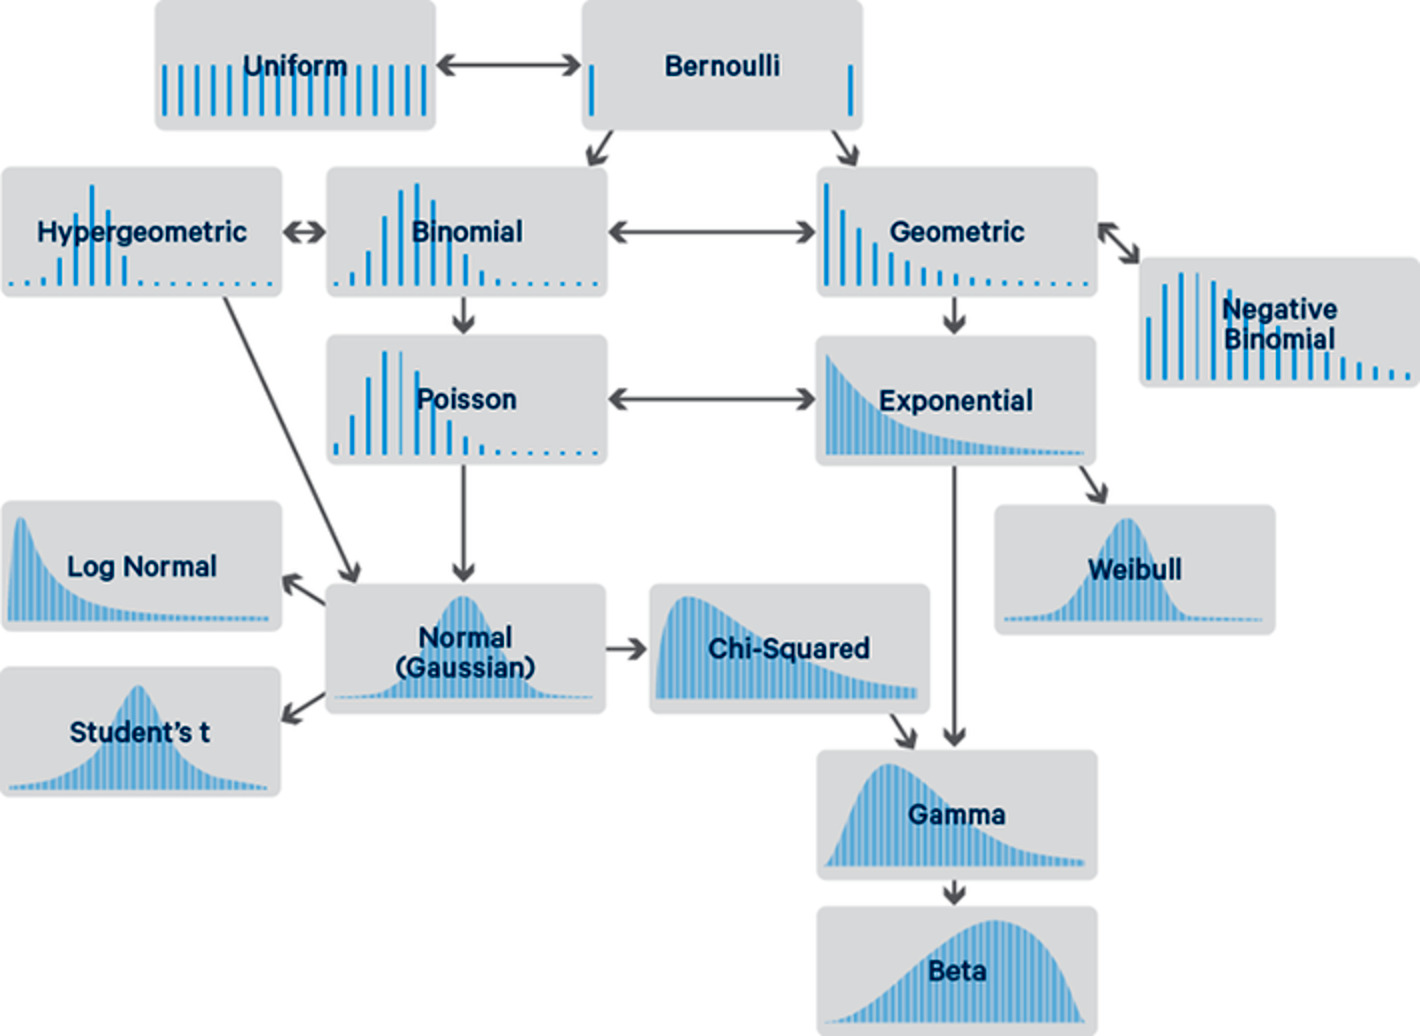
\includegraphics[scale=0.4]{models}
	\end{center}
\end{sidewaysfigure}

\subsection{Modello bernoulliano}
Il modello bernoulliano impone alle sue variabili aleatorie di avere specificazione binaria, cioè $D_X=\{0,1\}$ per qualunque variabile $X$.

Una variabile aleatoria bernoulliana di probabilità di successo ($X=1$) $p$ si indica con
\begin{equation*}
	X\sim B(p)
\end{equation*}
mentre il fallimento è rappresentato da $(X = 0)$\\
\footnotesize{Brutalmente: quando gli esiti sono binari: il fallimento è rappresentato da 0 ed il successo da 1, stiamo parlando di un modello di bernoulli)
\normalsize

\subsubsection{Funzione di massa di probabilità}
La funzione di massa di probabilità di una variabile aleatoria bernoulliana è
\begin{equation*}
	p_X(x)=P(X=x)=p^x(1-p)^{1-x}I_{\{0,1\}}(x)=\begin{cases}
		1-p \qquad & x=0               \\
		p \qquad   & x=1               \\
		0 \qquad   & \text{altrimenti}
	\end{cases}
\end{equation*}


\subsubsection{Valore atteso}
In analogia con la proprietà \ref{prop:indvalatt}, il valore atteso di una variabile aleatoria bernoulliana è $p$:
\begin{equation*}
	\ev{X} = p
\end{equation*}
E ovviamente
\begin{equation*}
	\ev{X^2}=\ev{X}
\end{equation*}


\subsubsection{Varianza}
In analogia con la proprietà \ref{prop:indvar}, la varianza di una variabile aleatoria bernoulliana è $p(1-p)$:
\begin{equation*}
	\var(X) = p(1-p)
\end{equation*}


\subsubsection{Funzione di ripartizione}
La funzione di ripartizione per variabili bernoulliane è ovviamente uguale a $0$ per $x<0$, $1-p$ per $0\leq x<1$ e $1$ per $x\geq 1$.



\subsection{Modello binomiale}
Il modello binomiale consiste in $n$ ripetizioni di un esperimento bernoulliano di probabilità $p$. Una variabile aleatoria binomiale corrisponde al numero di successi tra gli $n$ esperimenti.
\begin{equation*}
	X \sim B(n, p)\qquad D_X=\{0,1,\dots,n\}
\end{equation*}


\subsubsection{Funzione di massa di probabilità}
Per definizione:
\begin{equation*}
	p_X(i) = P(X=i)
\end{equation*}
Tale probabilità è l'intersezione degli eventi indipendenti che consistono nel successo dal primo all'$i$-esimo e insuccesso dall'$i+1$-esimo all'$n$-esimo. In quanto probabilità di eventi indipendenti, essa può essere espressa come il prodotto delle singole probabilità. Ognuna delle probabilità di successo, per come è costruito il modello binomiale, è $p$, mentre ognuna delle probabilità di insuccesso è $1-p$. Ogni combinazione in cui $i$ esperimenti hanno successo e $n-i$ falliscono è valida, perciò:
\begin{equation}
	P(X=i) = \binom{n}{i} p^i(1-p)^{n-i}
\end{equation}

Concorde con la \eqref{eq:sommamassa}, la somma delle immagini della funzione di massa di probabilità è 1:
\begin{equation*}
	\sum_{i=1}^n p_X(i) = \sum_{i=1}^n \binom{n}{i} p^i(1-p)^{n-i} = (p+1-p)^n = 1
\end{equation*}


\subsubsection{Valore atteso}
Essendo ogni variabile aleatoria binomiale la somma di variabili aleatorie bernoulliane:
\begin{equation}
	\ev{X} = \ev{\sum_{i=0}^n X_i} = \sum_{i=0}^n \ev{X_i} = \sum_{i=0}^n p = np
\end{equation}


\subsubsection{Varianza}
Essendo le componenti bernoulliane indipendenti:
\begin{equation}
	\var(X)=\sum_{i=1}^n \var(X_i) = \sum_{i=1}^n p(1-p) = np(1-p)
\end{equation}


\subsubsection{Funzione di ripartizione}
Per calcolare con un'unica formula la funzione di ripartizione si aggiungono due funzioni indicatrici, che agiscono se $x>n$:
\begin{align}
	F_X(x) & = P(X\leq x)                                                                           \nonumber            \\
	       & = I_{(n,+\infty)}(x) + I_{[0,n]}(x) \sum_{i=0}^{\floor{x}}\binom{n}{i} p^i (1-p)^{n-i} \label{eq:ripabinom} \\
	       & = \begin{cases}
		\sum_{i=0}^{\floor{x}}\binom{n}{i} p^i (1-p)^{n-i}\quad & x\leq n \\
		1                                                       & x>n     \\
	\end{cases} \nonumber
\end{align}

\subsubsection{Relazioni tra variabili binomiali}
Siano $X_1$ e $X_2$ due variabili aleatorie definite su modelli binomiali che differiscono solo per il numero di esperimenti:
\begin{align*}
	 & X_1\sim B(n, p)\quad & X_1=\sum_{i=1}^n X_{1,i}\qquad & X_{1,i}\sim B(p)~\forall i\in\{1,\dots,n\} \\
	 & X_2\sim B(m, p)\quad & X_1=\sum_{j=1}^m X_{2,j}\qquad & X_{2,j}\sim B(p)~\forall j\in\{1,\dots,m\}
\end{align*}

\noindent
Se $X_1$ e $X_2$ sono indipendenti, allora:
\begin{equation*}
	X_1+X_2 = \sum_{i=1}^n X_{1,i} + \sum_{j=1}^m X_{2,j} = \sum_{i=1}^{n+m} Y_i = Y
\end{equation*}
dove $Y\sim B(n+m, p)$.



\subsection{Modello uniforme discreto} \label{subsec:unifdisc}
Nel modello uniforme discreto le variabili aleatorie consistono nell'esito di un esperimento da $n$ esiti possibili equiprobabili:
\begin{equation*}
	X\sim U(n)
\end{equation*}


\subsubsection{Funzione di massa di probabilità}
Essendo gli $n$ esiti equiprobabili, la funzione di massa di probabilità assume il valore $\frac{1}{n}$ per tutti i valori dell'input compresi tra gli esiti (numerati qui da $1$ a $n$):
\begin{equation*}
	p_X(i) = P(X=i) = \frac{1}{n} I_{\{1,\dots,n\}}(i)
\end{equation*}


\subsubsection{Funzione di ripartizione}
\begin{equation*}
	\forall x\leq n\qquad F_X(x) = P(X\leq x) = \sum_{i=1}^{\floor{x}} P(X=i) = \sum{i=1}^{\floor{x}} \frac{1}{n} = \frac{\floor{x}}{n}
\end{equation*}
Come per la \eqref{eq:ripabinom}, si aggiungono funzioni indicatrici per regolare il valore oltre $n$:
\begin{equation}
	F_X(x)=\frac{\floor{x}}{n} I_{[1,n]}(x)+I_{(n,+\infty)}(x)
\end{equation}


\subsubsection{Valore atteso}
Banalmente, usando la definizione:
\begin{equation} \label{eq:disunvalat}
	\ev{X} = \sum_{i=1}^n i P(X=i) = \frac{1}{n} \sum_{i=1}^n i = \frac{1}{n}\frac{n(n+1)}{2} = \frac{n+1}{2}
\end{equation}


\begin{equation*}
	\ev{X^2} = \sum_{i=1}^{n}\frac{i^2}{n} = \frac{1}{n}\sum_{i=1}^{n}i^2=\frac{(n+1)(2n+1)}{6}
\end{equation*}


\subsubsection{Varianza}
Usando la definizione equivalente di varianza e quanto appena calcolato:
\begin{align*}
	\var(X) & = \ev{X^2} - \ev{X}^2 =                                       \bc{proprietà \ref{prop:varalt}}           \\
	        & = \sum_{i=1}^n i^2 P(X=i) - \left(\frac{n+1}{2}\right)^2      \bc{valore atteso e \eqref{eq:disunvalat}} \\
	        & = \frac{1}{n} \sum_{i=1}^n i^2 - \left(\frac{n+1}{2}\right)^2 \bc{ipotesi di equiprobabilità}            \\
	        & = \frac{(n+1)(2n+1)}{6}-\left(\frac{n+1}{2}\right)^2          \bc{somma notevole}                        \\
	        & = (n+1)\left(\frac{2n+1}{6}+\frac{n+1}{4}\right)              \bc{raccogliendo $n+1$}                    \\
	        & = (n+1)\left(\frac{n-1}{12}\right)                                                                       \\
	        & = \frac{n^2-1}{12}
\end{align*}



\subsection{Modello geometrico}
Una variabile aleatoria geometrica corrisponde al numero di insuccessi prima del primo successo in una sequenza di esperimenti bernoulliani con lo stesso parametro $p$ e tra loro indipendenti.

Per $p=0$ non si ottiene mai un successo, pertanto la variabile geometrica non è definita. Per $p=1$ la variabile assume necessariamente il valore $0$.

Il supporto di una variabile geometrica è l'insieme dei naturali.

\begin{equation*}
	X\sim G(p)\qquad D_X=\N
\end{equation*}


\subsubsection{Funzione di massa di probabilità}
La funzione di massa di probabilità in $i$ è uguale alla probabilità di insuccesso per ognuna delle $i$ ripetizioni indipendenti per la probabilità di successo della $i+1$-esima.

Come sempre si aggiunge una funzione indicatrice per aggiustare il dominio di $F_X$:
\begin{equation} \label{eq:geommasprob}
	F_X(i) = P(X=i) = (1-p)^ip ~ I_{N\cup\{0\}} (i)
\end{equation}

La somma delle immagini della funzione di massa di probabilità converge, come dovrebbe, a $1$:
\begin{align*}
	\sum_{i=0}^{+\infty} P(X=i) & = \sum_{i=0}^{+\infty} p(1-p)^i \\
	                            & = p\sum_{i=0}^{+\infty} (1-p)^i \\
	                            & = p\frac{1}{1-(1-p)}            \\
	                            & = 1
\end{align*}


\subsubsection{Valore atteso}
Tramite la definizione:
\begin{align*}
	\ev{X} & = \sum_{i=0}^{+\infty} i P(X=i)                    \bc{definizione \ref{def:valatt}}         \\
	       & = \sum_{i=0}^{+\infty} ip(1-p)^i                   \bc{\eqref{eq:geommasprob}}               \\
	       & = p(1-p)\sum_{i=0}^{+\infty} i(1-p)^{i-1}                                                    \\
	       & = -p(1-p) \frac{d}{dx} \sum_{i=0}^{+\infty} (1-p)^i \bc{derivata di $(1-p)^i$ e della somma} \\
	       & = -p(1-p) \frac{d}{dx} \frac{1}{p}                  \bc{serie geometrica di ragione $1-p$}   \\
	       & = \frac{p(1-p)}{p^2} = \frac{1-p}{p}                 \bc{derivando}
\end{align*}


\subsubsection{Varianza}
Volendo usare la forma equivalente \eqref{eq:varalt} di cui alla proprietà \ref{prop:varalt}, si calcola innanzitutto il valore atteso del quadrato della variabile:
\begin{align*}
	\ev{X^2} & = \sum_{i=0}^{+\infty} i^2 p(1-p)^i                                                                                                          \\
	         & = p(1-p) \sum_{i=0}^{+\infty} i^2 (1-p)^{i-1}                                                                                                \\
	         & = -p(1-p) \sum_{i=0}^{+\infty} i \frac{d}{dp}(1-p)^i \bc{derivata di $(1-p)^i$}                                                              \\
	         & = -p(1-p) \frac{d}{dp}\sum_{i=0}^{+\infty} i (1-p)^i \bc{\parbox{42.5mm}{prodotto di una derivata per una costante e derivata di una somma}} \\
	         & = -p(1-p) \frac{d}{dp}(1-p)\sum_{i=0}^{+\infty} i (1-p)^{i-1}                                                                                \\
	         & = p(1-p) \frac{d}{dp}(1-p) \frac{d}{dp} \sum_{i=0}^{+\infty} (1-p)^i                                                                         \\
	         & = -p(1-p) \frac{d}{dp} \frac{1-p}{p^2}                                                                                                       \\
	         & = -p(1-p) \frac{-p^2-2p(1-p)}{p^4}                                                                                                           \\
	         & = (1-p) \frac{p+2(1-p)}{p^2}                                                                                                                 \\
	         & = \frac{(1-p)(2-p)}{p^2}
\end{align*}
Da cui:
\begin{align*}
	\var(X) & = \ev{X^2}-\ev{X}^2                                     \\
	        & = \frac{(1-p)(2-p)}{p^2} - \left(\frac{1-p}{p}\right)^2 \\
	        & = \frac{(1-p)((2-p)-(1-p))}{p^2}                        \\
	        & = \frac{1-p}{p^2}
\end{align*}


\subsubsection{Funzione di ripartizione}
\begin{align*}
	F_X(n) & = P(X\leq n) = 1-P(X>n) =                                                                                                 \\
	       & = 1 - \sum_{i=n+1}^{+\infty} P(X=i)                                                                                       \\
	       & = 1 - \sum_{i=n+1}^{+\infty} p(1-p)^i                                                                                     \\
	       & = 1 - p(1-p)^{n+1} \sum_{i=n+1}^{+\infty} (1-p)^{i-(n+1)} \justif{~}{moltiplicando per $\frac{(1-p)^{n+1}}{(1-p)^{n+1}}$} \\
	       & = 1 - p(1-p)^{n+1} \sum_{i=0}^{+\infty} (1-p)^i \justif{~}{sostituzione: $i=i-(n+1)$}                                     \\
	       & = 1 - p(1-p)^{n+1} \frac{1}{1-(1-p)}                                                                                      \\
	       & = 1 - (1-p)^{n+1}                                                                                                         \\
\end{align*}
Questo risultato è in realtà banale se si applica il concetto semantico alla variabile geometrica.

\begin{equation*}
	F_X(x) = P(X\leq x) = 1-P(X>x) = 1-(1-p)^{\floor{x}+1}
\end{equation*}


\subsubsection{Assenza di memoria} \label{geom-assmem}
Come si può intuire, la probabilità di costante insuccesso all'$i+j$-esimo esperimento non è condizionata dalla probabilità di costante insuccesso all'$i$-esimo. Questo risultato prende il nome di assenza di memoria.
\begin{align*}
	P(X\geq i+j \mid X\geq i) & = \frac{P(X\geq i+j \cap X\geq i)}{P(X\geq i)} \\
	                          & = \frac{P(X\geq i+j)}{P(X\geq i)}              \\
	                          & = \frac{(1-p)^{i+j}}{(1-p)^i}                  \\
	                          & = (1-p)^j                                      \\
	                          & = P(X\geq j)
\end{align*}



\subsection{Modello di Poisson}
\begin{equation*}
	X\sim P(\lambda) \qquad D_X = \N \qquad \lambda>0
\end{equation*}

\subsubsection{Funzione di massa di probabilità}
\begin{equation*}
	P_X(i) = P(X=i) = e^{-\lambda}\frac{\lambda^i}{i!} ~ I_\N(i)
\end{equation*}

Ancora una volta la somma delle immagini della funzione di massa di probabilità converge a $1$:
\begin{equation} \label{eq:poisummas}
	\sum_{i=0}^{+\infty} e^{-\lambda}\frac{\lambda^i}{i!} = e^{-\lambda}\sum_{i=0}^{+\infty} \frac{\lambda^i}{i!} = e^{-\lambda}e^\lambda = 1
\end{equation}


\subsubsection{Valore atteso}
Tramite la definizione:
\begin{align}
	\ev{X} & = \sum_{i=0}^{+\infty} i P(X=i) = \sum_{i=1}^{+\infty} i P(X=i) \bc{definizione \ref{def:valatt}} \nonumber \\
	       & = \sum_{i=1}^{+\infty} i e^{-\lambda}\frac{\lambda^i}{i!} \label{eq:poinotevolelambda}                      \\
	       & = \lambda e^{-\lambda} \sum_{i=1}^{+\infty} \frac{\lambda^{i-1}}{(i-1)!} \nonumber                          \\
	       & = \lambda e^{-\lambda} \sum_{i=0}^{+\infty}\frac{\lambda^i}{i!} \bc{sostituzione: $i=i-1$} \nonumber        \\
	       & = \lambda e^{-\lambda} e^\lambda \nonumber                                                                  \\
	       & = \lambda
\end{align}


\subsubsection{Varianza}
Volendo usare la forma equivalente \eqref{eq:varalt}, si calcola innanzitutto il valore atteso di $X^2$:
\begin{align*}
	\ev{X^2} & = \sum_{i=1}^{+\infty} i^2 e^{-\lambda}\frac{\lambda^i}{i!}                                                                                                                              \\
	         & = \sum_{i=1}^{+\infty} i e^{-\lambda} \frac{\lambda^i}{(i-1)!}                                                                                                                           \\
	         & = \lambda\sum_{i=1}^{+\infty} i e^{-\lambda}\frac{\lambda^{i-1}}{(i-1)!}                                                                                                                 \\
	         & = \lambda\sum_{i=1}^{+\infty} (i-1+1) e^{-\lambda}\frac{\lambda^{i-1}}{(i-1)!}                                                                                                           \\
	         & = \lambda\sum_{i=1}^{+\infty}\left((i-1)e^{-\lambda}\frac{\lambda^{i-1}}{(i-1)!}+e^{-\lambda}\frac{\lambda^{i-1}}{(i-1)!}\right)                                                         \\
	         & = \lambda\sum_{i=1}^{+\infty} (i-1)e^{-\lambda}\frac{\lambda^{i-1}}{(i-1)!} + \lambda\sum_{i=1}^{+\infty} + e^{-\lambda}\frac{\lambda^{i-1}}{(i-1)!}                                     \\
	         & = \lambda\underbrace{\sum_{i=0}^{+\infty} ie^{-\lambda}\frac{\lambda^i}{i!}}_{\lambda} + \lambda \underbrace{\sum_{i=0}^{+\infty} e^{-\lambda}\frac{\lambda^i}{i!}}_{1} \bc{con $i=i-1$} \\
	         & = \lambda^2 + \lambda \bc{\eqref{eq:poinotevolelambda} e \eqref{eq:poisummas}}
\end{align*}
Ergo
\begin{align}
	\var(X) & = \ev{X^2} - \ev{X}^2         \nonumber \\
	        & = \lambda^2+\lambda-\lambda^2 \nonumber \\
	        & = \lambda
\end{align}

\subsubsection{Approssimazione del modello binomiale} \label{subsub:binompois}
Il modello di Poisson è strettamente legato al modello binomiale. Infatti, se il prodotto dei parametri di una binomiale è costante, per $n$ grandi essa è ben approssimata da una variabile di Poisson che ha come parametro tale prodotto:
\begin{equation*}
	X\sim B(n, p)\qquad\text{con }np=\lambda
\end{equation*}
Per $n\to+\infty$:
\begin{align*}
	P(X=i) & = \binom{n}{i} p^i (1-p)^{n-i}                                                                                                                                                                                                                                                \\
	       & = \binom{n}{i}\left(\frac{\lambda}{n}\right)^i\left(1-\frac{\lambda}{n}\right)^{n-i}                                                                                                                                                                                          \\
	       & = \frac{n(n-1) \dots (n-i+1)}{i!} \cdot \frac{\lambda^i}{n^i} \left( 1 - \frac{\lambda}{n} \right)^{n-i}                                                                                                                                                                      \\
	       & = \frac{n(n-1) \dots (n-i+1)}{n^i} \cdot \frac{\lambda^i}{i!} \left( 1 - \frac{\lambda}{n} \right)^{n-i}                                                                                                                                                                      \\
	       & = \underbrace{\frac{n}{n}}_{\to 1} \cdot \underbrace{\frac{n-1}{n}}_{\to 1} \dots \underbrace{\frac{n-i+1}{n}}_{\to 1} \cdot \frac{\lambda^i}{i!} \cdot \underbrace{\frac{\left( 1 - \frac{\lambda}{n} \right)^n}{\left( 1 - \frac{\lambda}{n} \right)^i}}_{\to e^{-\lambda}} \\
	       & \to \frac{\lambda^i}{i!} e^{-\lambda}
\end{align*}

\subsection{Riproducibilità}
\begin{center}
$x_1 \sim P (\lambda_1), x_2 \sim P(\lambda_2) \quad \rightarrow \quad x_1 + x_2 \sim P(\lambda_1 + \lambda_2)$
\end{center}


\subsection{Modello ipergeometrico}
Il modello ipergeometrico descrive il classico problema dell'urna. Dati $N$ oggetti funzionanti e $M$ oggetti difettosi, sia $n$ il numero di estrazioni senza reimmissione. La variabile aleatoria ipergeometrica X è il numero di oggetti funzionanti nelle $n$ estrazioni.
\begin{equation*}
	X\sim ?(?)
\end{equation*}
Il modello è valido solo se $P(X=0)=0$.

%todo: what is this


\subsubsection{Funzione di massa di probabilità}
Il numero di casi possibili sono le combinazioni di $n$ estrazioni senza reimmissione da un gruppo di $N+M$. Il numero di casi favorevoli si può calcolare applicando il principio fondamentale del calcolo combinatorio.
\begin{equation*}
	P(X=i) = \frac{\binom{N}{i}\binom{M}{n-i}}{\binom{N+M}{n}}
\end{equation*}


\subsubsection{Valore atteso}
Al fine di calcolare il valore atteso si sfrutta un approccio decomposizionale: si introducono $n$ variabili aleatorie $X_i$, ognuna legata a un'estrazione, tali che
\begin{equation*}
	X_i = \begin{cases}
		1 & \text{l'$i$-esimo oggetto estratto funziona} \\
		0 & \text{altrimenti}
	\end{cases}
\end{equation*}

Per tali variabili vale
\begin{equation*}
	P(X_i=1) = \frac{N}{N+M} =: p = \ev{X_i}
\end{equation*}

Da cui
\begin{align*}
	\ev{X} & = \ev{\sum_{i=1}^n X_i} \\
	       & = \sum_{i=1}^n \ev{X_i} \\
	       & = np
\end{align*}


\subsubsection{Varianza}
Applicando la proprietà \ref{prop:varalt} si calcola la varianza delle singole $X_i$:
\begin{align*}
	\var(X_i) & = \ev{X_i^2}-\ev{X_i}^2                                   \\
	          & = \ev{X_i}(1-\ev{X_i})          \bc{idempotenza di $X_i$} \\
	          & = \frac{N}{N+M} + \frac{M}{N+M}                           \\
	          & = \frac{NM}{(N+M)^2}
\end{align*}

Essendo le variabili $X_i$ non indipendenti, la varianza della loro somma non è uguale alla somma delle varianze. Si può comunque applicare la proprietà \ref{prop:varsumcov} e passare per le covarianze:
\begin{align*}
	\cov(X_i,X_j) & = \ev{X_i X_j} - \ev{X_i}\ev{X_j}                                \\
	              & = \ev{X_i=1\cap X_j=1} - \left(\frac{N}{N+M}\right)^2            \\
	              & = P(X_j=1 \mid X_i=1)P(X_i=1) - \left(\frac{N}{N+M}\right)^2     \\
	              & = \frac{N-1}{N+M-1} \frac{N}{N+M} - \left(\frac{N}{N+M}\right)^2 \\
	              & = \frac{N}{N+M} \left(\frac{N-1}{N+M-1} - \frac{N}{N+M}\right)   \\
	              & = \frac{-NM}{(N+M-1)(N+M)^2}
\end{align*}
Ergo
\begin{align*}
	\var(X) & = \sum_{i=1}^n \var(X_i) + \sum_{i\neq j}^n \cov(X_i,X_j)     \\
	        & = n\frac{NM}{(N+M)^2} - n(n-1)\cdot\frac{-NM}{(N+M-1)(N+M)^2} \\
	        & = n\frac{NM}{(N+M)^2}\left(1-(n-1)\frac{1}{N+M-1}\right)      \\
	        & = np(1-p)\left(1-\frac{n-1}{N+M-1}\right)
\end{align*}
Per $N+M\to+\infty$ il modello si semplifica in un modello binomiale:
\begin{equation*}
	\to np(1-p)
\end{equation*}


\subsection{Modello uniforme continuo}
Il modello uniforme continuo estende al continuo i concetti visti alla sezione \ref{subsec:unifdisc} per il modello uniforme discreto e viene determinato da un intervallo equivalentemente aperto o chiuso:
\begin{equation*}
	X \sim U([a,b]) \quad a < b \quad D_x = [a,b]
\end{equation*}


\subsubsection{Funzione di densità di probabilità}
\begin{equation*}
	f(X)(x) = \frac{1}{b-a} I[a,b](x)
\end{equation*}
essendo la densità costante, per $I\subseteq[a,b]$:
\begin{equation*}
	P(X\in I) = \frac{|I|}{b-a}
\end{equation*}
dove $|I|$ è la somma delle ampiezze $p-q$ degli intervalli disgiunti $[p,q]$ da cui $I$ è composto.

Come da definizione, integrando nell'intero $\R$ la funzione di densità di probabilità si ottiene $1$:
\begin{equation*}
	\int_{-\infty}^{+\infty}f_X(x) = \int_a^b\frac{1}{b-a}dx = \frac{1}{b-a} \eval{x}{a}{b} = 1
\end{equation*}


\subsubsection{Funzione di ripartizione}
Per definizione la funzione di ripartizione è la funzione integrale della funzione di densità:
\begin{align*}
	F_X(x) & = P(X\leq x)                   \\
	       & = \int_{-\infty}^x f_X(u)du    \\
	       & = \int_a^x \frac{1}{b-a}du     \\
	       & = \frac{1}{b-a} \eval{u}{a}{x} \\
	       & = \frac{x-a}{b-a}
\end{align*}
\footnotesize{}
$f_X(u)du$ perché la variabile non può essere uguale\\
\normalsize{}

Come sempre funzioni indicatrici aggiustano il risultato per punti non appartenenti all'intervallo:
\begin{equation*}
	F_X(x) = \frac{x-a}{b-a} I_{[a,b]}(x) + I_{(b,+\infty)}(x)
\end{equation*}


\subsubsection{Valore atteso}
Applicando la definizione:
\begin{align*}
	\ev{X} & = \int_a^b x f_X(x)dx                      \\
	       & = \frac{1}{b-a} \int_a^b x ~ dx            \\
	       & = \frac{1}{b-a} \eval{\frac{x^2}{2}}{a}{x} \\
	       & = \frac{1}{b-a} \cdot \frac{b^2-a^2}{2}    \\
	       & = \frac{b+a}{2}
\end{align*}
Che deriva dalla somma tra la area del rettangolo e l'area del triangolo nel grafico, che corrisponde anche al punto medio.


\subsubsection{Varianza}
Come di consueto si intende applicare la proprietà \ref{prop:varalt}, pertanto si calcola innanzitutto il valore atteso di $X^2$:
\begin{align*}
	\ev{X^2} & = \int_a^b x^2 f_X(x)dx                    \\
	         & = \frac{1}{b-a}\int_a^b x^2 ~ dx           \\
	         & = \frac{1}{b-a} \eval{\frac{x^3}{3}}{a}{b} \\
	         & = \frac{b^3-a^3}{3(b-a)}                   \\
	         & = \frac{a^2+ab+b^2}{3}
\end{align*}

E infine:
\begin{align*}
	\var(X) & = \ev{X^2} - \ev{X}^2                      \\
	        & = \frac{a^2+ab+b^2}{3} - \frac{(a+b)^2}{4} \\
	        & = \frac{(b-a)^2}{12}
\end{align*}


\subsection{Modello esponenziale}
Nel modello esponenziale la funzione di densità è esponenziale.
\begin{equation*}
	X\sim E(\lambda) \qquad \lambda\in\R^+ \quad D_X=\R^+
\end{equation*}


\subsubsection{Funzione di densità di probabilità}
\begin{equation*}
	f_X(x) = \lambda e^{-\lambda x} I_{\R^+}(x)
\end{equation*}

Il modello esponenziale si usa per modellare il tempo che intercorre tra due eventi.

La funzione di densità rispetta la definizione, infatti:
\begin{align*}
	\int_0^{+\infty} f_X(x)dx & = \int_0^{+\infty} \lambda e^{-\lambda x} dx       \\
	                          & = \int_0^{+\infty} e^{-y}dy \bc{con $y=\lambda x$} \\
	                          & = \eval{-e^{-y}}{0}{+\infty}                       \\
	                          & = 0 + e^{-0}                                       \\
	                          & = 1
\end{align*}


\subsubsection{Funzione di ripartizione}
Applicando la definizione di funzione di ripartizione continua:
\begin{align*}
	F_X(x) & = \int_0^x f_X(y)dy                                  \\
	       & = \int_0^x \lambda e^{\lambda y}dy                   \\
	       & = \int_0^{\lambda x} e^{-z}dz \bc{con $z=\lambda y$} \\
	       & = \eval{-e^{-z}}{0}{\lambda x}                       \\
	       & = -e^{-\lambda x} + e^0                              \\
	       & = 1-e^{-\lambda x}
\end{align*}
Aggiungendo una funzione indicatrice:
\begin{equation}
	F_X(x) = (1 - e^{-\lambda x})I_{\R^+}(x)
\end{equation}


\subsubsection{Valore atteso}
Applicando la definizione:
\begin{align*}
	\ev{X} & = \int_0^{+\infty} x f_X(x) dx                                                             \\
	       & = \int_0^{+\infty} x\lambda e^{-\lambda x}dx                                               \\
	       & = \eval{-x e^{-\lambda x}}{0}{+\infty} + \int_0^{+\infty} e^{-\lambda x} dx \bc{per parti} \\
	       & = \int_0^{+\infty} e^{-\lambda x} dx                                                       \\
	       & = \frac{1}{\lambda} \underbrace{\int_0^{+\infty} \lambda e^{-\lambda x}}_{1}               \\
	       & = \frac{1}{\lambda} \bc{proprietà di $f_X$}
\end{align*}


\subsubsection{Varianza}
Volendo usare la forma equivalente \eqref{eq:varalt}, si calcola innanzitutto il valore atteso di $X^2$:
\begin{align*}
	\ev{X^2} & = \int_0^{+\infty} x^2\lambda e^{-\lambda x} dx                                 \\
	         & = \eval{-x^2 e^{-\lambda x}}{0}{+\infty} + \int_0^{+\infty} 2xe^{-\lambda x} dx \\
	         & = 2\int_0^{+\infty} xe^{-\lambda x}dx                                           \\
	         & = \frac{2}{\lambda} \int_0^{+\infty} \lambda xe^{-\lambda x}dx                  \\
	         & = \frac{2}{\lambda} \ev{X} = \frac{2}{\lambda^2}
\end{align*}
Da cui:
\begin{align*}
	\var(X) & = \ev{X^2} - \ev{X}^2                                           \\
	        & = \frac{2}{\lambda^2}-\frac{1}{\lambda^2} = \frac{1}{\lambda^2}
\end{align*}


\subsubsection{Assenza di memoria}
Le variabili di modello esponenziale godono della proprietà di assenza di memoria (già vista per il modello geometrico al paragrafo \ref{geom-assmem}):
\begin{equation*}
	P(X>x) = 1 - F_X(x) = e^{-\lambda x}
\end{equation*}
Quindi:
\begin{align*}
	P(X>s+t) & = e^{-\lambda (s+t)}           \\
	         & = e^{-\lambda s}e^{-\lambda t} \\
	         & = P(X>s)P(X>t)
\end{align*}
Da cui
\begin{align*}
	P(X>s) & = \frac{P(X>s+t)}{P(X>t)}         \\
	       & = \frac{P(X>s+t\cap X>t)}{P(X>t)} \\
	       & = P(X>s+t\mid X>t)
\end{align*}
Le due espressioni coincidono logicamente. Possiamo estendere questa notazione:
\begin{align*}
P(x < x ) & = 1 - P(X \leq x ) = \\
		 & =1 - F_x = e ^{-\lambda x}
\end{align*}


\subsubsection{Corollario}
Consideriamo un modello esponenziale
\begin{center}
$X \sim E(\lambda) \quad Y := \alpha X \quad \alpha > 0$
\end{center}
\begin{align*}
F_y(x) &= P(Y \leq x) = P(\alpha X \leq x) = P(x \leq \frac{x}{\alpha})\\
	  & F_x(\frac{x}{\alpha}) = 1 - e^{-\lambda \frac{x}{\alpha}} = 1 - e ^{-\frac{\lambda}{\alpha}x}\\
	  & \lambda ' = \frac{\lambda}{\alpha} \quad F_y(x) = 1- e^{-\lambda ' x}\\
	  & Y \sim E(\frac{\lambda}{\alpha})
\end{align*}





\subsection{Risultati notevoli sui modelli}
\begin{prop}
	Siano $X_1,\dots,X_n$ variabili aleatorie indipendenti e sia $Y$ il massimo degli $X_i$, ossia $Y:=\max_i X_i$. Allora:
	\begin{equation*}
		F_Y(x) = \prod_{i=1}^n F_{X_i}(x)
	\end{equation*}
	E per variabili indipendenti e identicamente distribuite (i.i.d.) secondo una funzione di ripartizione $F$:
	\begin{equation*}
		F_Y(x) = \prod_{i=1}^n F(x) = F(x)^n
	\end{equation*}
\end{prop}
\begin{proof}
	\begin{equation*}
		F_Y(x) = P(Y\leq x) = P(\max_i X_i\leq x) = P(\forall i X_i\leq x)
	\end{equation*}
	Dal momento che gli $X_i$ sono indipendenti, l'ultima probabilità è uguale al prodotto delle singole:
	\begin{equation*}
		= \prod_{i=1}^n P(X_i \leq x) = \prod_{i=1}^n F_{X_i}(x)
	\end{equation*}
	Nell'ulteriore ipotesi di variabili indipendenti e identicamente distribuite (i.i.d.) secondo una funzione di ripartizione $F$:
	\begin{equation*}
		= \prod_{i=1}^n F(x) = F(x)^n
	\end{equation*}
\end{proof}

\begin{prop} \label{prop:modnotmin}
	Siano $X_1,\dots,X_n$ variabili aleatorie indipendenti e sia $Z$ il minimo degli $X_i$, ossia $Z:=\min_i X_i$. Allora:
	\begin{equation*}
		F_Z(x) = 1 - \prod_{i=1}^n (1-F_{X_i}(x))
	\end{equation*}
	E per variabili indipendenti e identicamente distribuite (i.i.d.) secondo una funzione di ripartizione $F$:
	\begin{equation*}
		F_Z(x) = 1 - (1-F(x))^n
	\end{equation*}
\end{prop}
\begin{proof}
	\begin{equation*}
		F_Z(x) = 1 - P(Z>x) = 1 - P(\min X_i > x) = 1 - P(\forall i X_i > x)
	\end{equation*}
	Dal momento che gli $X_i$ sono indipendenti, l'ultima probabilità è uguale al prodotto delle singole:
	\begin{equation*}
		= 1 - \prod_{i=1}^n P(X_i > x) = 1 - \prod_{i=1}^n (1-F_{X_i}(x))
	\end{equation*}
	Nell'ulteriore ipotesi di variabili indipendenti e identicamente distribuite (i.i.d.) secondo una funzione di ripartizione $F$:
	\begin{equation*}
		= 1 - \prod_{i=1}^n (1-F(x)) = 1 - (1-F(x))^n
	\end{equation*}
\end{proof}

\begin{prop}
	Siano $X_1,\dots,X_n$ variabili aleatorie indipendenti e sia $Z$ il minimo degli $X_i$, ossia $Z:=\min_i X_i$. Se $X_i\sim E(\lambda_i)$ per ogni $i$, allora:
	\begin{equation*}
		Z\sim E\left(\sum_{i=1}^n \lambda_i\right)
	\end{equation*}
\end{prop}
\begin{proof}
	Essendo le variabili esponenziali le loro funzioni di ripartizione sono del tipo:
	\begin{equation*}
		F_{X_i}(x) = 1-e^{-\lambda_i x}
	\end{equation*}
	Per la proprietà \ref{prop:modnotmin}:
	\begin{align*}
		F_Z(x) & = 1 - \prod_{i=1}^n (1-F_{X_i}(x))   \\
		       & = 1 - \prod_{i=1}^n e^{-\lambda_i x} \\
		       & = 1 - e^{\sum_{i=1}^n -\lambda_i x}  \\
		       & = 1 - e^{-x \sum_{i=1}^n \lambda_i}  \\
	\end{align*}
	Chiamato $\lambda = \sum_{i=1}^n \lambda_i$, allora $Z\sim E(\lambda)$:
	\begin{equation*}
		F_Z(x) = 1 - e^{-\lambda x}
	\end{equation*}
\end{proof}

\begin{prop}
	Se $X\sim E(\lambda)$ e $Y:=cX$ con $c\in\R^+$, allora $Y$ è una variabile aleatoria esponenziale di parametro $\frac{\lambda}{c}$.
	\begin{equation*}
		F_Y(x) = 1 - e^{-\frac{\lambda}{c} x}
	\end{equation*}
\end{prop}
\begin{proof}
	\begin{align*}
		F_Y(x) & =                                  \\
		       & = P(Y \leq x)                      \\
		       & = P(xC \leq x)                     \\
		       & = P\left(X \leq \frac{x}{c}\right) \\
		       & = F_X\left(\frac{x}{c}\right)      \\
		       & = 1 - e^{-\frac{\lambda}{c} x}     \\
	\end{align*}
\end{proof}

\subsection{Sistemi in serie}
I modelli di sistemi in serie rappresentano una serie di componenti che lavorano in maniera sequenziale tra loro, l'output di un modello rappresenta l'input del prossimo, fino al terminarsi della catena.
\begin{center}
$\rightarrow 1 \rightarrow 2 \rightarrow ... \rightarrow n \rightarrow$
\end{center}
Consideriamo 
\begin{align*}
x_i & = \text{istante in cui si rompe il componente}\quad  i \sim E(\lambda_i)\\
y_i & = \text{istante in cui il sistema smette di funzionare} \\
   & = min x_i  \sim E(\sum_{}{} \lambda_i)
\end{align*}
%Il modello esponenziale descrive bene questo modello (per motivi definiti più avanti






\subsection{Modello gaussiano (o normale)}
Una variabile $X$ di modello gaussiano (o normale), è una variabile aleatoria continua definita da due parametri:
\begin{equation*}
	X\sim N(\mu, \sigma)\qquad \mu\in\R,\sigma\in\R^+
\end{equation*}


\subsubsection{Funzione di densità di probabilità}
\begin{equation*}
	f_X(x) = \frac{1}{\sqrt{2\pi}~\sigma}e^{-\dfrac{(x-\mu)^2}{2\sigma^2}}
\end{equation*}

Studiando la funzione di densità si verifica algebricamente la famosa forma \qt{a campana}:
\begin{align*}
	 & \bullet \lim_{x\to\pm\infty} f_X(x) = 0                                                 \\
	 & \bullet f'_x(x) = \frac{1}{\sqrt{2\pi}~\sigma^3}e^{-\frac{(x-\mu)^2}{2\sigma^2}}(\mu-x) \\
	 & \bullet f'_x(x) \geq 0 \Leftrightarrow x\leq\mu                                         \\
	 & \bullet f''_x(x) = \left(\frac{x-\mu}{\sigma}\right)^2 - 1                              \\
	 & \bullet f''_x(x) \geq 0 \Leftrightarrow x\geq \mu+\sigma \lor x\leq \mu-\sigma
\end{align*}
Modificare $\mu$ significa ovviamente traslare la curva parallelamente all'asse delle $x$. Aumentare il valore di $\sigma$ significa diminuire l'ordinata del massimo e, conseguentemente, \qt{allargare la campana} (in quanto l'area totale sottesa deve rimanere invariata). Vale ovviamente il viceversa per una diminuzione.

Si può dimostrare che l'area sottesa alla funzione di densità è $1$:
\begin{equation*}
	\int_{-\infty}^{+\infty} \frac{1}{\sqrt{2\pi}~\sigma} e^{-\frac{1}{2}\left(\frac{x-\mu}{\sigma}\right)^2} dx = 1
\end{equation*}

\subsubsection{Funzione di ripartizione}
La funzione di ripartizione è una funzione liscia (integrabile infinite volte) e non possiede una forma analitica. 
\begin{equation*}
	F_X(x) = P( X \leq x) = \int_{-\infty}^x \frac{1}{\sqrt{2\pi}~\sigma} e^{-\frac{1}{2}\left(\frac{y-\mu}{\sigma}\right)^2} dy
\end{equation*}


\subsubsection{Valore atteso}
\begin{equation*}
	\ev{X} = \mu
\end{equation*}


\subsubsection{Varianza}
\begin{equation*}
	\var(X) = \sigma^2
\end{equation*}


\subsubsection{Distribuzione normale standard}
A partire da una variabile gaussiana $X$ si può costruire la variabile $Z$ come standardizzazione (normalizzazione) di $X$:
\begin{equation*}
	Z = \frac{x-\mu}{\sigma}
\end{equation*}

\noindent
Si verificano i seguenti risultati
\begin{align*}
	\ev{Z}  & = \ev{\frac{1}{\sigma}\ev{X-\mu}}  \\
	        & = \frac{1}{\sigma}(\ev{X}-\mu) = 0 \\
	\\
	\var(Z) & = \frac{1}{\sigma^2} \var(X-\mu)   \\
	        & = \frac{1}{\sigma^2}\var(X) = 1
\end{align*}
Ergo
\begin{equation*}
	X\sim N(\mu,\sigma) \Rightarrow Z\sim N(0,1)
\end{equation*}

Le variabili normali standard si indicano solitamente con $Z$, mentre le relative funzioni di densità e di ripartizione di indicano rispettivamente con $\phi(z)$ e $\Phi(z)$.


\subsubsection{Risultati notevoli}

\paragraph{Trasformazioni lineari} Trasformando linearmente la variabile aleatoria $X\sim N(\mu,\sigma)$, si ottiene una variabile aleatoria gaussiana $Y$:
\begin{equation*}
	X\sim N(\mu,\sigma) \Rightarrow Y\sim N(a\mu+b,a\sigma)
\end{equation*}
\begin{itemize}
\item Il valore atteso: $\ev{Y} = \ev{aX + b}  = a \ev{X} + b = a\mu + b$
\item La varianza: $var(Y ) = Var(ax + b) = a^2 var(x) = a^2\sigma^2$
\end{itemize}

\paragraph{Standardizzazione}
Consideriamo nuovamente una variabile aleatoria $X \sim N(\mu, \sigma)$ con:
\begin{equation*}
Z = \frac{x-\mu}{\sigma} = \frac{x}{\sigma} - \frac{\mu}{\sigma} \sim N(0, 1)
\end{equation*}
Con $S = \frac{R-\mu}{\sigma}$
\begin{itemize}
\item $\ev{R} = \mu \rightarrow \ev{s} = 0$
\item $var(R) = \sigma^2 \rightarrow var(S) = 1$ 
\end{itemize}



\paragraph{Riproducibilità} Date variabili $X_1,\dots,X_n$ gaussiane indipendenti tali che $\forall i X_i\sim N(\mu_i,\sigma_i)$:
\begin{equation*}
	Y\sim N\left(\sum_{i=1}^n \mu_i,\sqrt{\sum_{i=1}^n \sigma_i^2}\right)
\end{equation*}
Anche il modello binomiale e l'ipergeometrico, ad esempio, godono della proprietà di riproducibilità.

\paragraph{Funzione di ripartizione normale e standard} è possibile ricavare la funzione di ripartizione di una variabile aleatoria gaussiana qualsiasi conoscendo la funzione di ripartizione di una variabile standard:
\begin{align*}
	F_X(x) & = P(X\leq x)                                                 \\
	       & = P\left(\frac{X-\mu}{\sigma}\leq\frac{x-\mu}{\sigma}\right) \\
	       & = P\left(Z\leq \frac{x-\mu}{\sigma}\right)                   \\
	       & = F_Z\left(\frac{x-\mu}{\sigma}\right)                       \\
	       & = \Phi\left(\frac{x-\mu}{\sigma}\right)
\end{align*}
Questa tecnica può essere applicata anche per calcolare la probabilità tra due estremi:
\begin{align*}
P(\alpha \leq x \leq \beta) & = P(\frac{\alpha - \mu}{\sigma} \leq \frac{x - \mu}{\sigma} \leq \frac{\beta - \mu}{\sigma})  = \\
& = P( \frac{\alpha - \mu}{\sigma} \leq Z \leq \frac{\beta - \mu}{\sigma}) =\\
& = \phi(\frac{\beta - \mu}{\sigma} )- \phi (\frac{\alpha - \mu}{\sigma} )
\end{align*}


\subsubsection{Variabili multiple}
Consideriamo un modello con due variabili aleatorie $X_1, X_2$ indipendenti:
\begin{center}
$X_1 \sim N(\mu_1, \sigma_1)$ \quad $X_2 \sim N(\mu_2, \sigma_2)$
\end{center}
Il modello sarà come segue:
\begin{center}
$X_1 + X_2 \sim N( \mu_1 + \mu_2 , \sqrt{\sigma_1^2 + \sigma_2^2})$
\end{center}
\begin{itemize}
% controllare il valore atteso
\item $\ev{X_1 + X_2} =  \mu_1 + \mu_2$
\item $var(X_1 + X_2) = var(X_1) + var(X_2) = \sigma_1^2 + \sigma_2^2$
\end{itemize}

%\subsection{Risultati notevoli sui modelli}




\subsection{Teorema centrale del limite}
\begin{teor}
	Siano $X_1,\dots,X_n$ variabili aleatorie indipendenti e identicamente distribuite, ossia tali che $\forall i\quad\ev{X_i}=\mu\land\var(X_i)=\sigma^2$. Allora per $n$ grandi le variabili sono distribuite in modo approssimativamente\footnote{Il simbolo $\modsim$ indica l'appartenenza approssimativa a un modello.} normale:
	\begin{gather*}
		\sum_{i=1}^n X_i \modsim N(n\mu,\sqrt{n}\sigma) \\
	\end{gather*}
	O, standardizzando
	\begin{equation*}
		\frac{\sum_{i=1}^n X_i-n\mu}{\sqrt{n}\sigma} \modsim N(0,1)
	\end{equation*}
	Ovvero sia:
	\begin{equation*}
		\lim_{n\to+\infty} P\left(\frac{\sum_{i=1}^n X_i-n\mu}{\sqrt{n}\sigma}\leq x\right) = \Phi(x)
	\end{equation*}
\end{teor}

\subsection{Indici di variabili aleatorie}
\begin{defin}
	Data una variabile aleatoria $X$, la mediana di $X$ è un numero $m\in\R$ tale che $P(X\leq m) = P(X>m) = 1/2$.
\end{defin}

\begin{defin}
	Data una variabile aleatoria $X$, la moda di $X$ è la specificazione di densità (o massa di probabilità) massima.
\end{defin}

% TODO: questa definizione va sistemata: una specificazione come quella descritta non è unica: come ci si comporta?
\begin{defin}
	Data una variabile aleatoria $X$, il quantile di livello $q\in[0,1]$ di $X$ è la specificazione $x_q\in\R$ tale che $P(X\leq x_q) = q$.

	\begin{center}
		$P(X \leq X_q) = q$\\
		$F_x (X_q) = q$ \\
		$X_q = F_x ^{-1}(F_x(X_q)) = F_x^{-1}(q)$
		
		\end{center}
\end{defin}



\subsubsection{Funzione cumulativa empirica}
La funzione cumulativa empirica dà una misura del numero di osservazioni che superano un dato input:
\begin{equation*}
	\hat F(x) = \frac{1}{n} \sum_{i=1}^n I_{(-\infty,x]}(x_i)
\end{equation*}
% TODO: check
Fatta una selezione di osservazioni sul campione, a patto che tale selezione sia coerente con la funzione di densità/massa, la funzione cumulativa empirica è un'approssimazione tanto più buona della funzione di ripartizione della selezione quanto grande è la selezione sul campione.

Per il teorema centrale del limite, variabili aleatorie bernoulliane di parametri alti possono essere approssimate con il modello normale:
\begin{gather*}
	X\sim B(n,p) \\
	X = \sum_{i=1}^n X_i \modsim N(np, \sqrt{np(1-p)}) \\
	\frac{x-np}{\sqrt{np(1-p)})} \modsim N(0,1)
\end{gather*}

%% Copyright (C) 2021 Alessandro Clerici Lorenzini
%
% This work may be distributed and/or modified under the
% conditions of the LaTeX Project Public License, either version 1.3
% of this license or (at your option) any later version.
% The latest version of this license is in
%   http://www.latex-project.org/lppl.txt
% and version 1.3 or later is part of all distributions of LaTeX
% version 2005/12/01 or later.
%
% This work has the LPPL maintenance status `maintained'.
%
% The Current Maintainer of this work is Alessandro Clerici Lorenzini
%
% This work consists of the files listed in work.txt


\section{Statistica inferenziale}
La statistica inferenziale tenta di applicare un'inferenza attraverso l'induzione. La statistica inferenziale riprende concetti della statistica descrittiva ma li reinterpreta in senso probabilistico applicando l'induzione.

\subsection{Definizioni}
Gli attori fondamentali della statistica inferenziale sono la popolazione, il campione la statistica o stimatore\footnote{in alcuni contesti, i termini statistica e stimatore differiscono leggermente di significato. Tuttavia in questo testo verranno usati equivalentemente.}, e la stima.

\begin{itemize}
	\item La popolazione è descritta come una \emph{variabile aleatoria $X$}. La branca della statistica inferenziale in cui la distribuzione di $X$ è nota a meno di uno o più parametri $\theta$ si dice \emph{parametrica}: $X\sim F(\theta)$. Se anche il modello della distribuzione è ignoto, si tratta di statistica inferenziale non parametrica. Nel resto di questo testo si studierà la statistica inferenziale parametrica;
	\item Poiché non sempre si vuole ricavare o approssimare il parametro di distribuzione ignoto $\theta$, ma talvolta un valore che ne deriva, si introduce la funzione $\tau(\theta)$ a indicare tale valore;
	\item L'informazione conosciuta sulla popolazione è data da un \emph{campione}, talvolta espresso come una serie di variabili aleatorie $X_1,\dots,X_n$ indipendenti e identicamente distribuite, talvolta come una tupla di loro specificazioni $x_1,\dots,x_n$;
	\item L'operazione di stimare $\tau(\theta)$ consiste nella statistica o stimatore, che è una funzione $t$ che associa a una tupla possibili specificazioni del campione a un numero reale che stima il valore cercato: $t:D_X^n\to\R$. Essendo la statistica una variabile aleatoria, la si rappresenta talvolta (quando si vuole evidenziare tale lettura) con $T$;
	\item Una stima $\hat\tau$ è un'immagine della statistica e approssima $\tau(\theta)$: $\hat\tau = t(x_1,\dots,x_n)$ con istanze $X_1=x_1,\dots,X_n=x_n$.
\end{itemize}

\subsubsection{Stimatori non deviati (o  distorto)}
\begin{defin}[stimatore non deviato]
	Uno stimatore $t$ è non deviato per una quantità $\tau(\theta)$ quando il suo valore atteso è uguale a $\tau(\theta)$:
	\begin{equation*}
		\ev{t(X_1,\dots,X_n)} = \tau(\theta)
	\end{equation*}
\end{defin}
Uno stimatore non è deviato quando non è soggetto ad un bias.

\begin{examp}
	Uno stimatore non deviato per stimare il valore atteso, indipendentemente dalla distribuzione, è quello che fa corrispondere alle specificazioni date la loro media:
	\begin{equation*}
		t(x_1,\dots,x_n) = \frac{1}{n} \sum_{i=1}^n x_i \qquad \tau(\theta) = \ev{X}
	\end{equation*}
	Infatti:
	\begin{align*}
		\ev{t} & = \ev{\frac{1}{n} \sum_{i=1}^n X_i} \\
		       & = \frac{1}{n}\sum_{i=1}^n \ev{X_i}  \\
		       & = \frac{1}{n} \cdot n\ev{X_i}       \\
		       & = \ev{X}
	\end{align*}
	Inoltre, calcolando la varianza dello stimatore ci si accorge che essa tende a 0 per campioni molto grandi:
	\begin{equation*}
		\var\left(\frac{1}{n} \sum_{i=1}^n X_i\right) = \frac{1}{n^2} \sum_{i=1}^n \var(X_i) = \frac{n}{n^2}\var(X) = \frac{\var(X)}{n}
	\end{equation*}
\end{examp}


\subsection{Errore quadratico medio}
Il errore quadratico medio (Mean Square Error o MSE) è un modo di valutare uno stimatore di una quantità ignota:
\begin{defin}[errore quadratico medio]
	\begin{equation*}
		\MSE_{\tau(\theta)}(T) = \ev{(T-\tau(\theta))^2}
	\end{equation*}
	con $T=t(X_1,\dots,X_n)$.
\end{defin}

\begin{defin}
	Il bias di uno stimatore $T$ su $\tau(\theta)$ è la differenza tra il suo valore atteso e $\tau(\theta)$:
	\begin{equation*}
		b_{T(\theta)}(T) = \ev{T} - \tau(\theta)
	\end{equation*}
\end{defin}

In virtù delle definizioni di MSE e bias si può trarre un interessante risultato:
\begin{align*}
	\MSE_{\tau(\theta)}(T) & = \ev{(T-\tau(\theta))^2}                                                                            \\
	                       & = \ev{(T-\ev{T}+\ev{T}-\tau(\theta))^2}                                                              \\
	                       & = \ev{(T-\ev{T})^2+2(T-\ev{T})(\ev{T}-\tau(\theta))+(\ev{T}-\tau(\theta))^2}                         \\
	                       & = \ev{(T-\ev{T})^2} + 2(\ev{T}-\tau(\theta))\underbrace{\ev{T-\ev{T}}}_{0} + (\ev{T}-\tau(\theta))^2 \\
	                       & = \var(T) + (\ev{T}-\tau(\theta))^2                                                                  \\
	                       & = \var(T) + (b_{T(\theta)}(T))^2
\end{align*}
Per definizione, se $T$ è uno stimatore non deviato per $\tau(\theta)$ allora $b_{\tau(\theta)}(T)=0$ e quindi l'errore quadratico medio di $T$ è uguale alla sua varianza.


\subsection{Stimatori consistenti}
\begin{defin}[Stimatore consistente in media quadratica]
	Uno stimatore $T_n$\footnote{Più precisamente, si parla di una famiglia di stimatori $T_n$ i cui membri differiscono per dimensione del campione} è consistente in media quadratica per $\tau(\theta)$ (tau) se
	\begin{equation*}
		\lim_{n\to+\infty} \MSE_{\tau(\theta)}(T_n) = 0
	\end{equation*}
\end{defin}

\begin{defin}[Stimatore debolmente consistente]
	Uno stimatore $T_n=t(X_1,\dots,X_n)$ è debolmente consistente rispetto a una quantità ignota $\tau(\theta)$ se e solo se
	\begin{equation*}
		\forall\varepsilon>0 \quad \lim_{n\to+\infty} P(\tau(\theta)-\varepsilon \leq T_n \leq \tau(\theta)+\varepsilon) = 1
	\end{equation*}
\end{defin}

%\footnotesize{}
%dato un \tau(\theta) fissato, dopo un valore  \epsilon, il valore sarà consistente

\begin{teor}
	Se uno stimatore $T$ è consistente in media quadratica per $\tau(\theta)$ allora $T$ è debolmente consistente per $\tau(\theta)$.
\end{teor}
\begin{proof}
	\begin{align*}
		P(-\varepsilon\leq T_n-\tau(\theta)\leq \varepsilon) & = P(\abs{T_n-\tau(\theta)}\leq\varepsilon)                                                                         \\
		                                                     & = P((T_n-\tau(\theta))^2\leq\varepsilon^2)                                                                         \\
		                                                     & = 1 - P((T_n-\tau(\theta))^2>\varepsilon^2)                                                                        \\
		                                                     & > 1-\frac{\ev{(T_n-\tau(\theta))^2}}{\varepsilon^2} \bc{\parbox{35mm}{disuguaglianza \ref{teor:markov} di Markov}} \\
		                                                     & = 1-\frac{\MSE_{\tau(\theta)}(T_n)}{\varepsilon^2} \to 1
	\end{align*}
	Essendo le probabilità limitate superiormente da $1$, per il teorema del confronto la probabilità iniziale tende a $1$.
\end{proof}


\subsection{Legge dei grandi numeri}
La legge dei grandi numeri forte ci dice che, date $n$ osservazioni con $n$ che tende ad infinito, lo stimatore media campionaria converge quasi certamente (ovvero $P = 1$) al valore atteso comune del $X_i$.
\begin{teor}[legge dei grandi numeri forte]
	\begin{equation*}
		P( \lim_{n\to+\infty} \bar X_n = \mu )= 1
	\end{equation*}
\end{teor}
Così come nella definizione di consistenza, possiamo definire la legge dei grandi numeri debole come:

\begin{teor}[legge dei grandi numeri debole]
	\begin{equation*}
		\forall\varepsilon > 0 \qquad \lim_{n\to+\infty} P\left(\abs{\bar X_n - \mu} > \varepsilon\right) = 0
	\end{equation*}
\end{teor}

%Ragionamento sulla deviazione standard campionaria, e $n-1$
% non si può derivare l'assenza di deviazione di s a partire da s^2

%Consideriamo:
%\begin{center}
%Popolazione $x$ \quad campione $x_1, ..., x_n$ \quad $\ev{x} = \mu$ \quad $var(x) = %\sigma^2$
%\end{center}
%E di voler stimare $\sigma^2$. La varianza campionaria è definita come:
%\begin{equation*}
%s^2 = \frac{1}{n-1} \sum_{i=1}^{n} (x_i - \bar x)^2 \quad \ev{s^2} = \sigma^2
%\end{equation*}
%\begin{enumerate}
%\item $\sum_{i=1}^{n} (x_i - \bar x)^2 = \sum_i x_i^2- n\bar x^2$
%\item $\ev{x^2} = var(x) + \ev{x}^2$
%\item $\ev{\bar x} = \mu , var(\bar x) = \frac{\sigma}{n}$
%\end{enumerate}
%...... 




\subsection{Problema dello scarto}
Un problema tipo che fa uso del teorema centrale del limite nella statistica inferenziale è il seguente.

Sia $\bar X_n$ la media campionaria dipendente da $n$ elementi e sia $\mu$ il suo valore atteso. Si vuole che lo scarto $\abs{\bar X_n - \mu}$ tra i due valori sia minore di una soglia $r$ (o solitamente $\epsilon$) con probabilità superiore a $1-\delta$ (con $\delta$ piccolo a piacere):
\begin{equation*}
	P(\abs{\bar X_n - \mu} \leq r) \geq 1-\delta \\
\end{equation*}

Normalizzando:
\begin{align*}
	P\left(\frac{\abs{\bar X_n - \mu}}{\sigma/\sqrt{n}} \leq \frac{r}{\sigma/\sqrt{n}}\right) & = P\left(\abs{\frac{\bar X_n - \mu}{\sigma/\sqrt{n}}} \leq \frac{r\sqrt{n}}{\sigma}\right)               \\
	                                                                                          & \approx P\left(\abs{Z} \leq \frac{r}{\sigma}\sqrt{n}\right)                                              \\
	                                                                                          & = P\left(-\frac{r}{\sigma}\sqrt{n}\leq Z\leq \frac{r}{\sigma}\sqrt{n}\right)                             \\
	                                                                                          & = \Phi\left(\frac{r}{\sigma}\sqrt{n}\right) - \Phi\left(- \frac{r}{\sigma}\sqrt{n}\right)                \\
	                                                                                          & = \Phi\left(\frac{r}{\sigma}\sqrt{n}\right) - \left(1 - \Phi\left(\frac{r}{\sigma}\sqrt{n}\right)\right)
\end{align*}

Ergo:
\begin{align*}
	2\Phi\left(\frac{r}{\sigma}\sqrt{n}\right) - 1 & \geq 1 - \delta                                                              \\
	\Phi\left(\frac{r}{\sigma}\sqrt{n}\right)      & \geq 1 - \frac{\delta}{2}                                                    \\
	\frac{r}{\sigma}\sqrt{n}                       & \geq \Phi^{-1}\left(1-\frac{\delta}{2}\right)                                \\
	n                                              & \geq \left(\frac{\sigma}{r}\Phi^{-1}\left(1-\frac{\delta}{2}\right)\right)^2
\end{align*}

Allo stesso modo si possono ricavare gli altri parametri del problema:
\begin{gather*}
	r \geq \frac{\sigma}{\sqrt{n}}\Phi^{-1}\left(1-\frac{\delta}{2}\right) \\
	\delta \geq 2\left(1-\Phi\left(\frac{r}{\sigma}\sqrt{n}\right)\right)
\end{gather*}
% TODO: verificare che $\sqrt{s^2}$ sia uno stimatore non deviato per $\sigma$
Mentre $\sigma$ tipicamente è stimato come $\sqrt{s^2}$ (dove $s$ è la deviazione standard campionaria).
\subsubsection{Variante con Tchebishev}
Consideriamo una variabile aleatoria $X$, con valore atteso: $\ev{X} = \mu$ e varianza: $var(X) = \sigma^2$:
Un'alternativa a questo tipo di stima si può fare applicando la disuguaglianza di Tchebishev:
\begin{equation*}
 P(\abs{X - \mu} < r) = 1- P(\abs{x-\mu} \geq r) \geq 1 - \frac{\sigma^2}{r^2}
\end{equation*}
% TODO: r=\varepsilon, coerenza a riguardo
% TODO: avere più uniformità tra i due metodi
Ne consegue che:
\begin{align*}
	\forall r > 0 \qquad P(\abs{X-\mu}\geq r)                                                       & \leq \frac{\sigma^2}{r^2}     \\
	P(\abs{X-\mu} < r) = 1-P(\abs{X-\mu}\geq r)                                & \geq 1 - \frac{\sigma^2}{r^2} \\
	P(\abs{\bar X-\mu} < \varepsilon) \geq 1 - \frac{\sigma^2}{n\varepsilon^2} & \geq 1-\delta                 \\
	\frac{\sigma^2}{n\varepsilon^2}                                            & \leq \delta                   \\
\end{align*}
% TODO: spiegazione
\begin{gather*}
	n \geq \frac{\sigma^2}{\delta\varepsilon^2} \Rightarrow P(\abs{\bar X-\mu}<\varepsilon) \geq 1-\delta \\
	\delta\geq\frac{\sigma^2}{n\varepsilon^2} \\[1ex]
	\varepsilon^2 \geq \frac{\sigma^2}{n\varepsilon} \rightarrow \varepsilon \geq \sqrt{\frac{\sigma^2}{n\delta}}
\end{gather*}

\subsubsection*{Per riassumere}
Con teorema centrale del limite: 
\begin{align*}
n 	& \geq \frac{\sigma^2}{\varepsilon^2} \Phi^{-1}(1-\frac{\delta}{2})^2 \\
 	& \geq \frac{\sigma^2}{\varepsilon^2} \Phi^{-1} (1-\frac{\delta}{2})^2 < \frac{\sigma^2}{\delta \varepsilon^2}\\
	& \geq \Phi^{-1} (1-\frac{\delta}{2})^2 < \frac{\sigma^2}{\delta}
\end{align*}
con Tchebishev:
\begin{align*}
	n & \geq \frac{\sigma^2}{\delta \varepsilon^2}\\
	 & \geq \Phi^{-1} ( 1 - \frac{\delta}{2})^2 < \frac{1}{\delta}
\end{align*}

Il metodo di Tchebishev è preferibile quando si vuole evitare approssimazioni, tuttavia rappresenta una approssimazione più lasca rispetto al metodo con teorema centrale del limite in quanto deve essere sempre valido.

% TODO: tutta la sezione sul processo di Poisson va rivista.
% TODO: definizione di processo stocastico

\subsection{Processo di Poisson}
Il processo di Poisson dimostra che sotto certe ipotesi il problema del numero di eventi che avvengono in un certo intervallo di tempo è descritto da un modello di Poisson.

\subsubsection{Processo stocastico}
\begin{teor}
	Sia $t$ una variabile temporale e $N(t)$ la variabile aleatoria che esprime il numero di eventi che avvengono nell'intervallo di tempo $[0,t)$. 
	\end{teor}
Possiamo dire che \begin{equation*}
	\{N(t): t > 0\} 
	\end{equation*}
	
	rappresenta un processo stocastico. Se estendiamo questa definizione con le seguenti ipotesi, possiamo dire che è anche un "processo di Poisson":\begin{center} con $\lambda > 0$
	\end{center}
	\begin{enumerate}
		\item $N(0)=0$;
		\item istanze di $N$ sono indipendenti per intervalli disgiunti, di conseguenza sono anche variabili aleatore indipendenti;
		\item la distribuzione del numero degli eventi dipende solo dalla lunghezza dell'intervallo di tempo (e non dalla loro posizione);
		      % TODO: spiegare la versione approssimata dell'ipotesi 3
		\item $\displaystyle\lim_{h\to0}\frac{P(N(h)=1)}{h}=\lambda$;\footnote{di conseguenza se $h$ è "piccolo" : $P(N(h) = 1) = \lambda h$}
		\item $\displaystyle\lim_{h\to0}\frac{P(N(h)\geq 2)}{h}=0$.\footnote{per $^6$, $P(N(h) \geq 2) = 0$}


	\end{enumerate}
	allora $N(t)$ è distribuita secondo il modello di Poisson con parametro $\lambda t$:
	\begin{equation*}
		N(t)\sim P(\lambda t)
	\end{equation*}

\begin{proof}
	Volendo calcolare la massa di probabilità $P(N(t)=k)$, si sceglie $n\in\N$ e si divide l'intervallo $[0,t)$ in $n$ parti uguali $[\frac{m}{n}t,\frac{m+1}{n}t)$. Potendo scegliere $n$ grande a piacere si può scegliere in particolare $n>k$.

	L'evento $N(t)=k \in \mathbb{N}$, di cui si vuole calcolare la probabilità, è esprimibile come l'unione disgiunta di due eventi:
	\begin{itemize}
		\item $A$: ognuno dei $k$ eventi avviene in un intervallo diverso, ossia: ogni intervallo contiene al più un evento, per un totale di $k$ eventi;
		\item $B$: esiste almeno un intervallo che contiene due eventi, per un totale di $k$ eventi.
	\end{itemize}
	e quindi:
	\begin{equation*}
		N(t)=k \in \mathbb{N} \leftrightarrow (A) \cup (B)
	\end{equation*}
	Ricordando che $n$ è grande a piacere, per l'ipotesi 4 la probabilità che uno specifico intervallo contenga due eventi tende a $0$. 
	Inoltre, per l'ipotesi 2 la probabilità dell'evento $B$ è calcolabile come il prodotto delle singole. 
	
	La probabilità complessiva è quindi il prodotto di fattori tendenti a $0$ ed è pertanto tendente a $0$ per $n\to+\infty$. Si ha quindi:
	\begin{align*}
		P(N(t)=k) & = P (A \cup B) = P(A) +  \xcancel{P(B)}\\
				& = \binom{n}{k} (\lambda \frac{t}{n})^k (1 - \lambda \frac{t}{n})^{n-k}
	\end{align*}
e quindi:
\begin{equation*}
	N(t) \sim B(n, \frac{\lambda t}{n})
\end{equation*}


Poiché il prodotto dei parametri della binomiale trovata è costante, ed essendo $n\to+\infty$, per quanto visto al paragrafo \ref{subsub:binompois} la distribuzione è ben descritta da un modello di Poisson di parametro $\lambda t$:
	\begin{equation*}
		N(t) \sim P(\lambda t)
	\end{equation*}

Per riassumere, con $n \rightarrow \infty$:
\begin{equation*}
	P(N(t) = k) = \frac{(\lambda t)^k}{k!} e^{-\lambda t}\quad I_{\mathbb{N} \cup \{0\}^{(k)}} 
\end{equation*}

%Inoltre:
%\begin{equation*}
 %P(nessun evento in (s, s+t\] = P (nessun evento in (0, t\] = 
 %P(N(t) = 0) = e^{-\lambda t}
%\end{equation*}

-----------


	Siano $B_i$ le variabili aleatorie bernoulliane che descrivono l'esistenza o meno di un evento nell'$i$-esimo intervallo. Per l'ipotesi 3 si ha, per $n\to+\infty$:
	\begin{equation*}
		B_i \sim B\left(\lambda\frac{t}{n}\right)
	\end{equation*}
	Si noti inoltre che l'evento $A$ corrisponde a una particolare specificazione della variabile aleatoria binomiale $B'$ che descrive il numero di eventi complessivi in $n$ intervalli, ossia la somma dei $B_i$:
	\begin{equation*}
		B'\sim B\left(n, \lambda\frac{t}{n}\right)
	\end{equation*}

	Ma allora:
	\begin{gather*}
		P(N(t)=k) = P(A) = P(B'=k) \\
		N(t) = B'
	\end{gather*}

	
	% TODO: esponenziale per il tempo trascorso da un evento all'altro
\end{proof}


\end{document}
